\documentclass[twoside]{book}

% Packages required by doxygen
\usepackage{fixltx2e}
\usepackage{calc}
\usepackage{doxygen}
\usepackage{graphicx}
\usepackage[utf8]{inputenc}
\usepackage{makeidx}
\usepackage{multicol}
\usepackage{multirow}
\PassOptionsToPackage{warn}{textcomp}
\usepackage{textcomp}
\usepackage[nointegrals]{wasysym}
\usepackage[table]{xcolor}

% Font selection
\usepackage[T1]{fontenc}
\usepackage{mathptmx}
\usepackage[scaled=.90]{helvet}
\usepackage{courier}
\usepackage{amssymb}
\usepackage{sectsty}
\renewcommand{\familydefault}{\sfdefault}
\allsectionsfont{%
  \fontseries{bc}\selectfont%
  \color{darkgray}%
}
\renewcommand{\DoxyLabelFont}{%
  \fontseries{bc}\selectfont%
  \color{darkgray}%
}
\newcommand{\+}{\discretionary{\mbox{\scriptsize$\hookleftarrow$}}{}{}}

% Page & text layout
\usepackage{geometry}
\geometry{%
  a4paper,%
  top=2.5cm,%
  bottom=2.5cm,%
  left=2.5cm,%
  right=2.5cm%
}
\tolerance=750
\hfuzz=15pt
\hbadness=750
\setlength{\emergencystretch}{15pt}
\setlength{\parindent}{0cm}
\setlength{\parskip}{0.2cm}
\makeatletter
\renewcommand{\paragraph}{%
  \@startsection{paragraph}{4}{0ex}{-1.0ex}{1.0ex}{%
    \normalfont\normalsize\bfseries\SS@parafont%
  }%
}
\renewcommand{\subparagraph}{%
  \@startsection{subparagraph}{5}{0ex}{-1.0ex}{1.0ex}{%
    \normalfont\normalsize\bfseries\SS@subparafont%
  }%
}
\makeatother

% Headers & footers
\usepackage{fancyhdr}
\pagestyle{fancyplain}
\fancyhead[LE]{\fancyplain{}{\bfseries\thepage}}
\fancyhead[CE]{\fancyplain{}{}}
\fancyhead[RE]{\fancyplain{}{\bfseries\leftmark}}
\fancyhead[LO]{\fancyplain{}{\bfseries\rightmark}}
\fancyhead[CO]{\fancyplain{}{}}
\fancyhead[RO]{\fancyplain{}{\bfseries\thepage}}
\fancyfoot[LE]{\fancyplain{}{}}
\fancyfoot[CE]{\fancyplain{}{}}
\fancyfoot[RE]{\fancyplain{}{\bfseries\scriptsize 2014年12月25日(木) 15時07分25秒作成 -\/ Validate / 構成\+:  Doxygen }}
\fancyfoot[LO]{\fancyplain{}{\bfseries\scriptsize 2014年12月25日(木) 15時07分25秒作成 -\/ Validate / 構成\+:  Doxygen }}
\fancyfoot[CO]{\fancyplain{}{}}
\fancyfoot[RO]{\fancyplain{}{}}
\renewcommand{\footrulewidth}{0.4pt}
\renewcommand{\chaptermark}[1]{%
  \markboth{#1}{}%
}
\renewcommand{\sectionmark}[1]{%
  \markright{\thesection\ #1}%
}

% Indices & bibliography
\usepackage{natbib}
\usepackage[titles]{tocloft}
\setcounter{tocdepth}{3}
\setcounter{secnumdepth}{5}
\makeindex

% Hyperlinks (required, but should be loaded last)
\usepackage{ifpdf}
\ifpdf
  \usepackage[pdftex,pagebackref=true]{hyperref}
\else
  \usepackage[ps2pdf,pagebackref=true]{hyperref}
\fi
\hypersetup{%
  colorlinks=true,%
  linkcolor=blue,%
  citecolor=blue,%
  unicode%
}

% Custom commands
\newcommand{\clearemptydoublepage}{%
  \newpage{\pagestyle{empty}\cleardoublepage}%
}


%===== C O N T E N T S =====

\begin{document}

% Titlepage & ToC
\hypersetup{pageanchor=false,
             bookmarks=true,
             bookmarksnumbered=true,
             pdfencoding=unicode
            }
\pagenumbering{roman}
\begin{titlepage}
\vspace*{7cm}
\begin{center}%
{\Large Validate }\\
\vspace*{1cm}
{\large 構築\+: Doxygen 1.8.8}\\
\vspace*{0.5cm}
{\small 2014年12月25日(木) 15時07分25秒}\\
\end{center}
\end{titlepage}
\clearemptydoublepage
\tableofcontents
\clearemptydoublepage
\pagenumbering{arabic}
\hypersetup{pageanchor=true}

%--- Begin generated contents ---
\chapter{階層索引}
\section{クラス階層}
この継承一覧はおおまかにはソートされていますが、完全にアルファベット順でソートされてはいません。\begin{DoxyCompactList}
\item \contentsline{section}{\-Rule\-Base}{\pageref{class_rule_base}}{}
\begin{DoxyCompactList}
\item \contentsline{section}{\-Rule\-Byte}{\pageref{class_rule_byte}}{}
\item \contentsline{section}{\-Rule\-Comparison}{\pageref{class_rule_comparison}}{}
\item \contentsline{section}{\-Rule\-Credit}{\pageref{class_rule_credit}}{}
\item \contentsline{section}{\-Rule\-Date}{\pageref{class_rule_date}}{}
\item \contentsline{section}{\-Rule\-Hiragana}{\pageref{class_rule_hiragana}}{}
\item \contentsline{section}{\-Rule\-Integer}{\pageref{class_rule_integer}}{}
\item \contentsline{section}{\-Rule\-Katakana}{\pageref{class_rule_katakana}}{}
\item \contentsline{section}{\-Rule\-Length}{\pageref{class_rule_length}}{}
\item \contentsline{section}{\-Rule\-Mail}{\pageref{class_rule_mail}}{}
\item \contentsline{section}{\-Rule\-Multi}{\pageref{class_rule_multi}}{}
\item \contentsline{section}{\-Rule\-Number}{\pageref{class_rule_number}}{}
\item \contentsline{section}{\-Rule\-Regular\-Expression}{\pageref{class_rule_regular_expression}}{}
\item \contentsline{section}{\-Rule\-Required}{\pageref{class_rule_required}}{}
\item \contentsline{section}{\-Rule\-Select}{\pageref{class_rule_select}}{}
\item \contentsline{section}{\-Rule\-Single}{\pageref{class_rule_single}}{}
\item \contentsline{section}{\-Rule\-Tel}{\pageref{class_rule_tel}}{}
\item \contentsline{section}{\-Rule\-Time}{\pageref{class_rule_time}}{}
\item \contentsline{section}{\-Rule\-Zip}{\pageref{class_rule_zip}}{}
\end{DoxyCompactList}
\item \contentsline{section}{\-Validate}{\pageref{class_validate}}{}
\item \contentsline{section}{\-Zip}{\pageref{class_zip}}{}
\end{DoxyCompactList}

\chapter{データ構造索引}
\section{データ構造}
データ構造一覧です。\begin{DoxyCompactList}
\item\contentsline{section}{\hyperlink{class_rule_base}{Rule\+Base} }{\pageref{class_rule_base}}{}
\item\contentsline{section}{\hyperlink{class_rule_byte}{Rule\+Byte} }{\pageref{class_rule_byte}}{}
\item\contentsline{section}{\hyperlink{class_rule_comparison}{Rule\+Comparison} }{\pageref{class_rule_comparison}}{}
\item\contentsline{section}{\hyperlink{class_rule_credit}{Rule\+Credit} }{\pageref{class_rule_credit}}{}
\item\contentsline{section}{\hyperlink{class_rule_date}{Rule\+Date} }{\pageref{class_rule_date}}{}
\item\contentsline{section}{\hyperlink{class_rule_hiragana}{Rule\+Hiragana} }{\pageref{class_rule_hiragana}}{}
\item\contentsline{section}{\hyperlink{class_rule_integer}{Rule\+Integer} }{\pageref{class_rule_integer}}{}
\item\contentsline{section}{\hyperlink{class_rule_katakana}{Rule\+Katakana} }{\pageref{class_rule_katakana}}{}
\item\contentsline{section}{\hyperlink{class_rule_length}{Rule\+Length} }{\pageref{class_rule_length}}{}
\item\contentsline{section}{\hyperlink{class_rule_mail}{Rule\+Mail} }{\pageref{class_rule_mail}}{}
\item\contentsline{section}{\hyperlink{class_rule_multi}{Rule\+Multi} }{\pageref{class_rule_multi}}{}
\item\contentsline{section}{\hyperlink{class_rule_number}{Rule\+Number} }{\pageref{class_rule_number}}{}
\item\contentsline{section}{\hyperlink{class_rule_regular_expression}{Rule\+Regular\+Expression} }{\pageref{class_rule_regular_expression}}{}
\item\contentsline{section}{\hyperlink{class_rule_required}{Rule\+Required} }{\pageref{class_rule_required}}{}
\item\contentsline{section}{\hyperlink{class_rule_select}{Rule\+Select} }{\pageref{class_rule_select}}{}
\item\contentsline{section}{\hyperlink{class_rule_single}{Rule\+Single} }{\pageref{class_rule_single}}{}
\item\contentsline{section}{\hyperlink{class_rule_tel}{Rule\+Tel} }{\pageref{class_rule_tel}}{}
\item\contentsline{section}{\hyperlink{class_rule_time}{Rule\+Time} }{\pageref{class_rule_time}}{}
\item\contentsline{section}{\hyperlink{class_rule_zip}{Rule\+Zip} }{\pageref{class_rule_zip}}{}
\item\contentsline{section}{\hyperlink{class_validate}{Validate} }{\pageref{class_validate}}{}
\item\contentsline{section}{\hyperlink{class_zip}{Zip} }{\pageref{class_zip}}{}
\end{DoxyCompactList}

\chapter{データ構造詳解}
\hypertarget{class_rule_base}{
\section{クラス \-Rule\-Base}
\label{class_rule_base}\index{\-Rule\-Base@{\-Rule\-Base}}
}
\-Rule\-Baseに対する継承グラフ\begin{figure}[H]
\begin{center}
\leavevmode
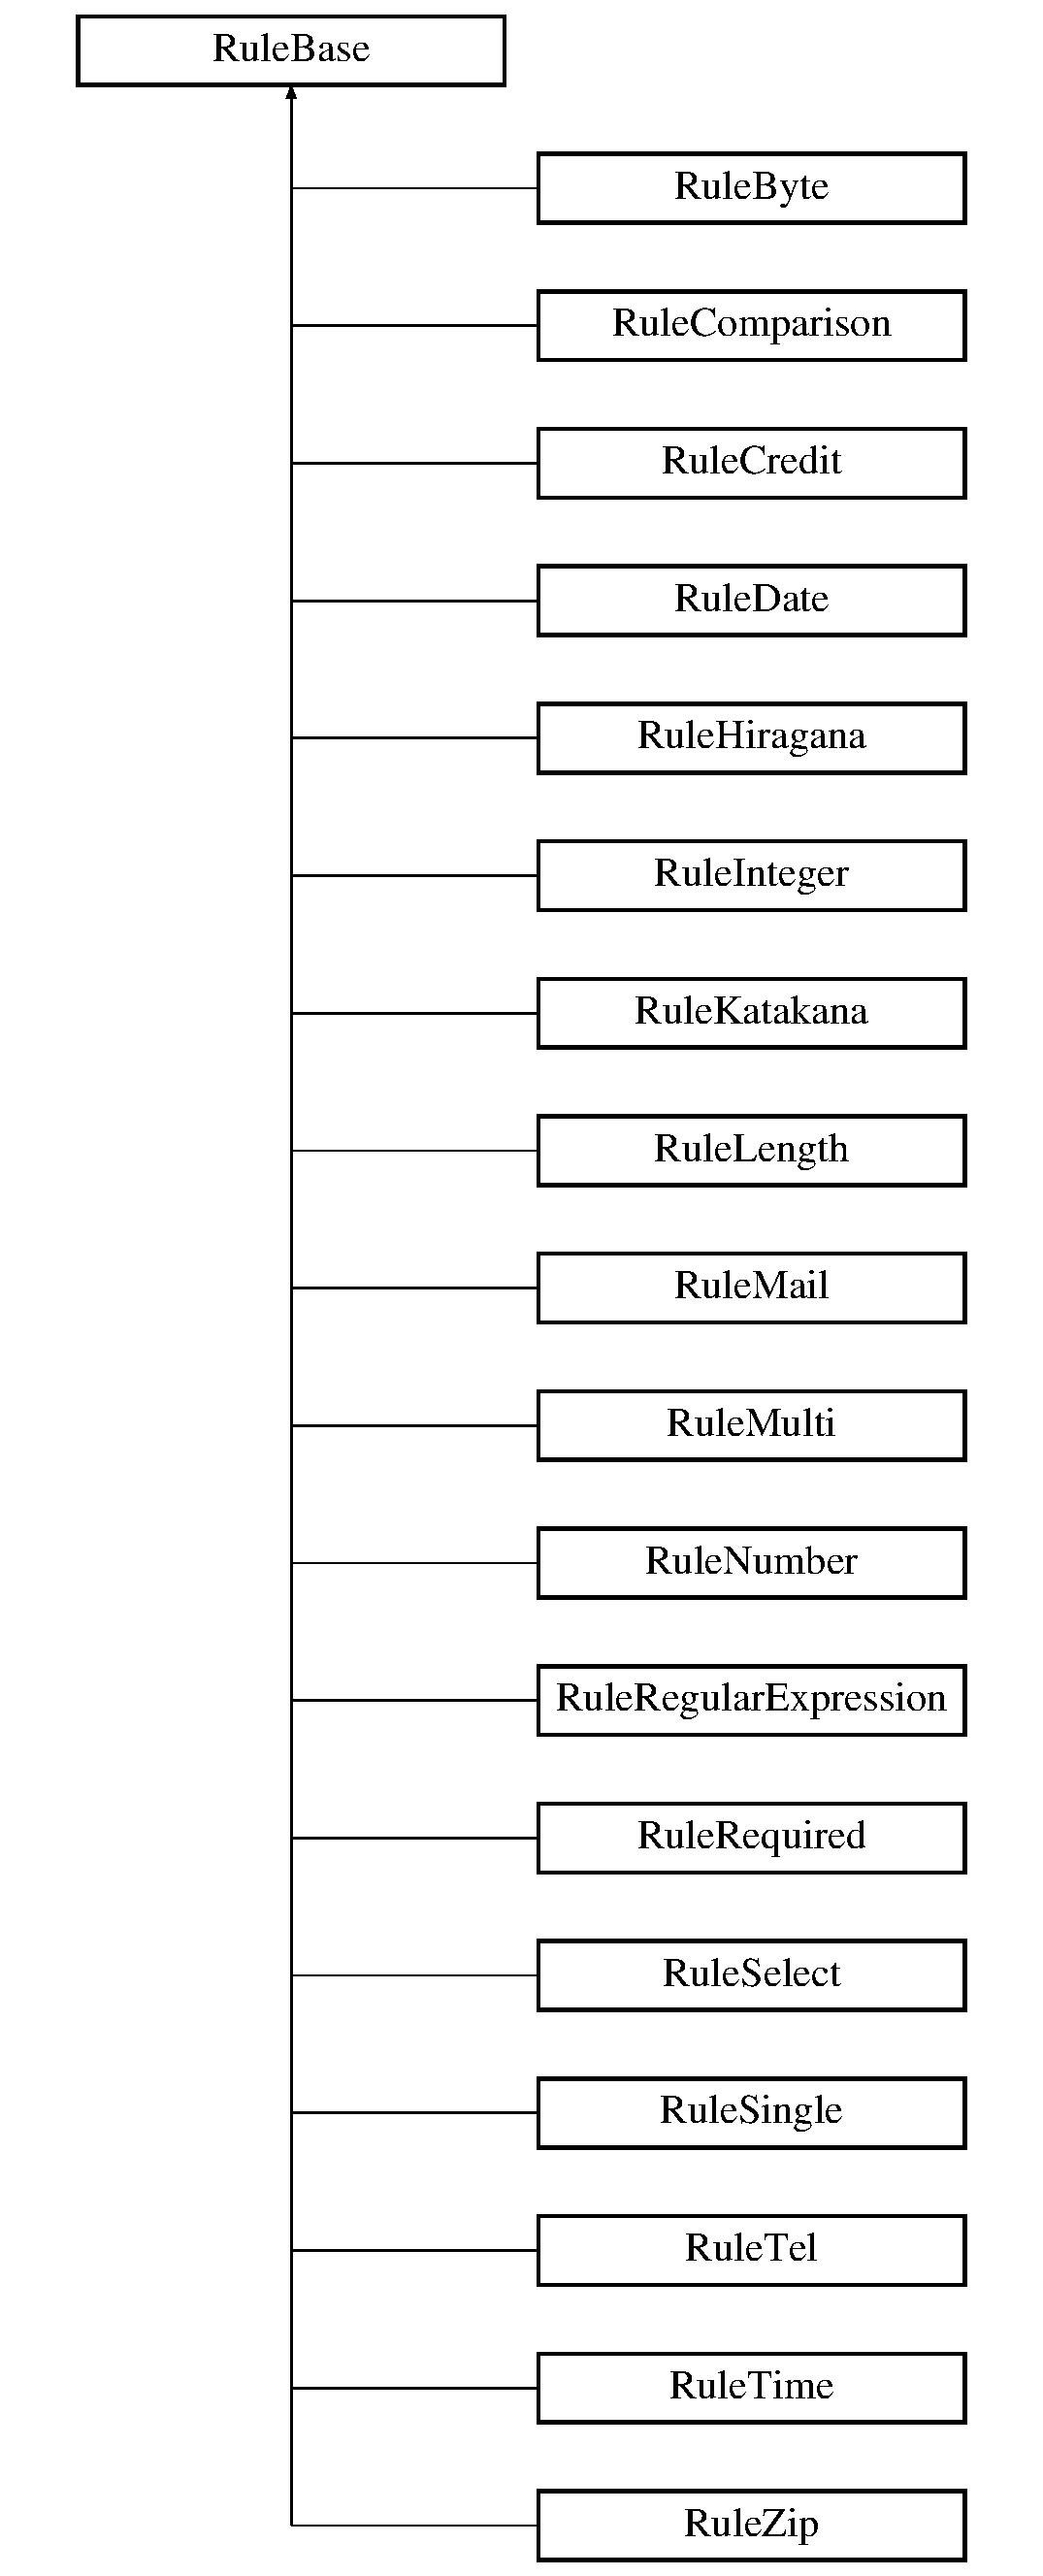
\includegraphics[height=12.000000cm]{class_rule_base}
\end{center}
\end{figure}
\subsection*{\-Public メソッド}
\begin{DoxyCompactItemize}
\item 
\hyperlink{class_rule_base_a7fdd69956610727a5a36b4f020bcf115}{\-\_\-\-\_\-construct} (\$file\-Nm)
\item 
\hyperlink{class_rule_base_a70eef3a06fda47704282eda5ea2706d9}{prepara} ()
\item 
\hyperlink{class_rule_base_afb0fafe7e02a3ae1993c01c19fad2bae}{run} ()
\end{DoxyCompactItemize}
\subsection*{変数}
\begin{DoxyCompactItemize}
\item 
\hyperlink{class_rule_base_a28d7688bd020a3b104adc19d1e08df96}{\$requests}
\end{DoxyCompactItemize}
\subsection*{\-Protected 変数}
\begin{DoxyCompactItemize}
\item 
\hyperlink{class_rule_base_a0f298096f322952a72a50f98a74c7b60}{\$value}
\item 
\hyperlink{class_rule_base_af24aefa35fa703a1521c8145fe8fa082}{\$infos}
\item 
\hyperlink{class_rule_base_ab7baba555b2cbc79c5ff9ef47baee3d5}{\$inies}
\end{DoxyCompactItemize}


\subsection{説明}
基底ルールクラス

\begin{DoxyVersion}{バージョン}
1.\-0.\-0  \-U\-T\-F-\/8  2011/10/05  2011/10/19 
\end{DoxyVersion}
\begin{DoxyAuthor}{作者}
mamiya\-\_\-shou 
\end{DoxyAuthor}
\begin{DoxyCopyright}{\-Copyright}
mamiya\-\_\-shou  \-M\-I\-T \-License  \-P\-H\-P 5.\-0 以上必須 
\end{DoxyCopyright}


\subsection{コンストラクタとデストラクタ}
\hypertarget{class_rule_base_a7fdd69956610727a5a36b4f020bcf115}{
\index{\-Rule\-Base@{\-Rule\-Base}!\-\_\-\-\_\-construct@{\-\_\-\-\_\-construct}}
\index{\-\_\-\-\_\-construct@{\-\_\-\-\_\-construct}!RuleBase@{\-Rule\-Base}}
\subsubsection[{\-\_\-\-\_\-construct}]{\setlength{\rightskip}{0pt plus 5cm}\-\_\-\-\_\-construct (
\begin{DoxyParamCaption}
\item[{\$}]{file\-Nm}
\end{DoxyParamCaption}
)}}
\label{class_rule_base_a7fdd69956610727a5a36b4f020bcf115}
コンストラクタ

public \begin{DoxyReturn}{戻り値}
void 
\end{DoxyReturn}


\subsection{関数}
\hypertarget{class_rule_base_a70eef3a06fda47704282eda5ea2706d9}{
\index{\-Rule\-Base@{\-Rule\-Base}!prepara@{prepara}}
\index{prepara@{prepara}!RuleBase@{\-Rule\-Base}}
\subsubsection[{prepara}]{\setlength{\rightskip}{0pt plus 5cm}prepara (
\begin{DoxyParamCaption}
{}
\end{DoxyParamCaption}
)}}
\label{class_rule_base_a70eef3a06fda47704282eda5ea2706d9}
バリデーション準備

public 
\begin{DoxyParams}{引数}
{\em array} & 可変長引数 \\
\hline
\end{DoxyParams}
\begin{DoxyReturn}{戻り値}
void 
\end{DoxyReturn}
\hypertarget{class_rule_base_afb0fafe7e02a3ae1993c01c19fad2bae}{
\index{\-Rule\-Base@{\-Rule\-Base}!run@{run}}
\index{run@{run}!RuleBase@{\-Rule\-Base}}
\subsubsection[{run}]{\setlength{\rightskip}{0pt plus 5cm}run (
\begin{DoxyParamCaption}
{}
\end{DoxyParamCaption}
)\hspace{0.3cm}{\ttfamily  \mbox{[}abstract\mbox{]}}}}
\label{class_rule_base_afb0fafe7e02a3ae1993c01c19fad2bae}
バリデートする

public  抽象メソッド 

\hyperlink{class_rule_mail_afb0fafe7e02a3ae1993c01c19fad2bae}{\-Rule\-Mail}, \hyperlink{class_rule_hiragana_afb0fafe7e02a3ae1993c01c19fad2bae}{\-Rule\-Hiragana}, \hyperlink{class_rule_katakana_afb0fafe7e02a3ae1993c01c19fad2bae}{\-Rule\-Katakana}, \hyperlink{class_rule_byte_afb0fafe7e02a3ae1993c01c19fad2bae}{\-Rule\-Byte}, \hyperlink{class_rule_comparison_afb0fafe7e02a3ae1993c01c19fad2bae}{\-Rule\-Comparison}, \hyperlink{class_rule_date_afb0fafe7e02a3ae1993c01c19fad2bae}{\-Rule\-Date}, \hyperlink{class_rule_multi_afb0fafe7e02a3ae1993c01c19fad2bae}{\-Rule\-Multi}, \hyperlink{class_rule_regular_expression_afb0fafe7e02a3ae1993c01c19fad2bae}{\-Rule\-Regular\-Expression}, \hyperlink{class_rule_single_afb0fafe7e02a3ae1993c01c19fad2bae}{\-Rule\-Single}, \hyperlink{class_rule_tel_afb0fafe7e02a3ae1993c01c19fad2bae}{\-Rule\-Tel}, \hyperlink{class_rule_time_afb0fafe7e02a3ae1993c01c19fad2bae}{\-Rule\-Time}, \hyperlink{class_rule_zip_afb0fafe7e02a3ae1993c01c19fad2bae}{\-Rule\-Zip}, \hyperlink{class_rule_credit_afb0fafe7e02a3ae1993c01c19fad2bae}{\-Rule\-Credit}, \hyperlink{class_rule_integer_afb0fafe7e02a3ae1993c01c19fad2bae}{\-Rule\-Integer}, \hyperlink{class_rule_length_afb0fafe7e02a3ae1993c01c19fad2bae}{\-Rule\-Length}, \hyperlink{class_rule_number_afb0fafe7e02a3ae1993c01c19fad2bae}{\-Rule\-Number}, \hyperlink{class_rule_required_afb0fafe7e02a3ae1993c01c19fad2bae}{\-Rule\-Required}, と \hyperlink{class_rule_select_afb0fafe7e02a3ae1993c01c19fad2bae}{\-Rule\-Select}で再定義されています。



\subsection{構造体}
\hypertarget{class_rule_base_af24aefa35fa703a1521c8145fe8fa082}{
\index{\-Rule\-Base@{\-Rule\-Base}!\$infos@{\$infos}}
\index{\$infos@{\$infos}!RuleBase@{\-Rule\-Base}}
\subsubsection[{\$infos}]{\setlength{\rightskip}{0pt plus 5cm}\$infos\hspace{0.3cm}{\ttfamily  \mbox{[}protected\mbox{]}}}}
\label{class_rule_base_af24aefa35fa703a1521c8145fe8fa082}
\hypertarget{class_rule_base_ab7baba555b2cbc79c5ff9ef47baee3d5}{
\index{\-Rule\-Base@{\-Rule\-Base}!\$inies@{\$inies}}
\index{\$inies@{\$inies}!RuleBase@{\-Rule\-Base}}
\subsubsection[{\$inies}]{\setlength{\rightskip}{0pt plus 5cm}\$inies\hspace{0.3cm}{\ttfamily  \mbox{[}protected\mbox{]}}}}
\label{class_rule_base_ab7baba555b2cbc79c5ff9ef47baee3d5}
\hypertarget{class_rule_base_a28d7688bd020a3b104adc19d1e08df96}{
\index{\-Rule\-Base@{\-Rule\-Base}!\$requests@{\$requests}}
\index{\$requests@{\$requests}!RuleBase@{\-Rule\-Base}}
\subsubsection[{\$requests}]{\setlength{\rightskip}{0pt plus 5cm}\$requests}}
\label{class_rule_base_a28d7688bd020a3b104adc19d1e08df96}
\hypertarget{class_rule_base_a0f298096f322952a72a50f98a74c7b60}{
\index{\-Rule\-Base@{\-Rule\-Base}!\$value@{\$value}}
\index{\$value@{\$value}!RuleBase@{\-Rule\-Base}}
\subsubsection[{\$value}]{\setlength{\rightskip}{0pt plus 5cm}\$value\hspace{0.3cm}{\ttfamily  \mbox{[}protected\mbox{]}}}}
\label{class_rule_base_a0f298096f322952a72a50f98a74c7b60}


このクラスの説明は次のファイルから生成されました\-:\begin{DoxyCompactItemize}
\item 
rules/\hyperlink{base__rule_8php}{base\-\_\-rule.\-php}\end{DoxyCompactItemize}

\hypertarget{class_rule_byte}{
\section{クラス \-Rule\-Byte}
\label{class_rule_byte}\index{\-Rule\-Byte@{\-Rule\-Byte}}
}
\-Rule\-Byteに対する継承グラフ\begin{figure}[H]
\begin{center}
\leavevmode
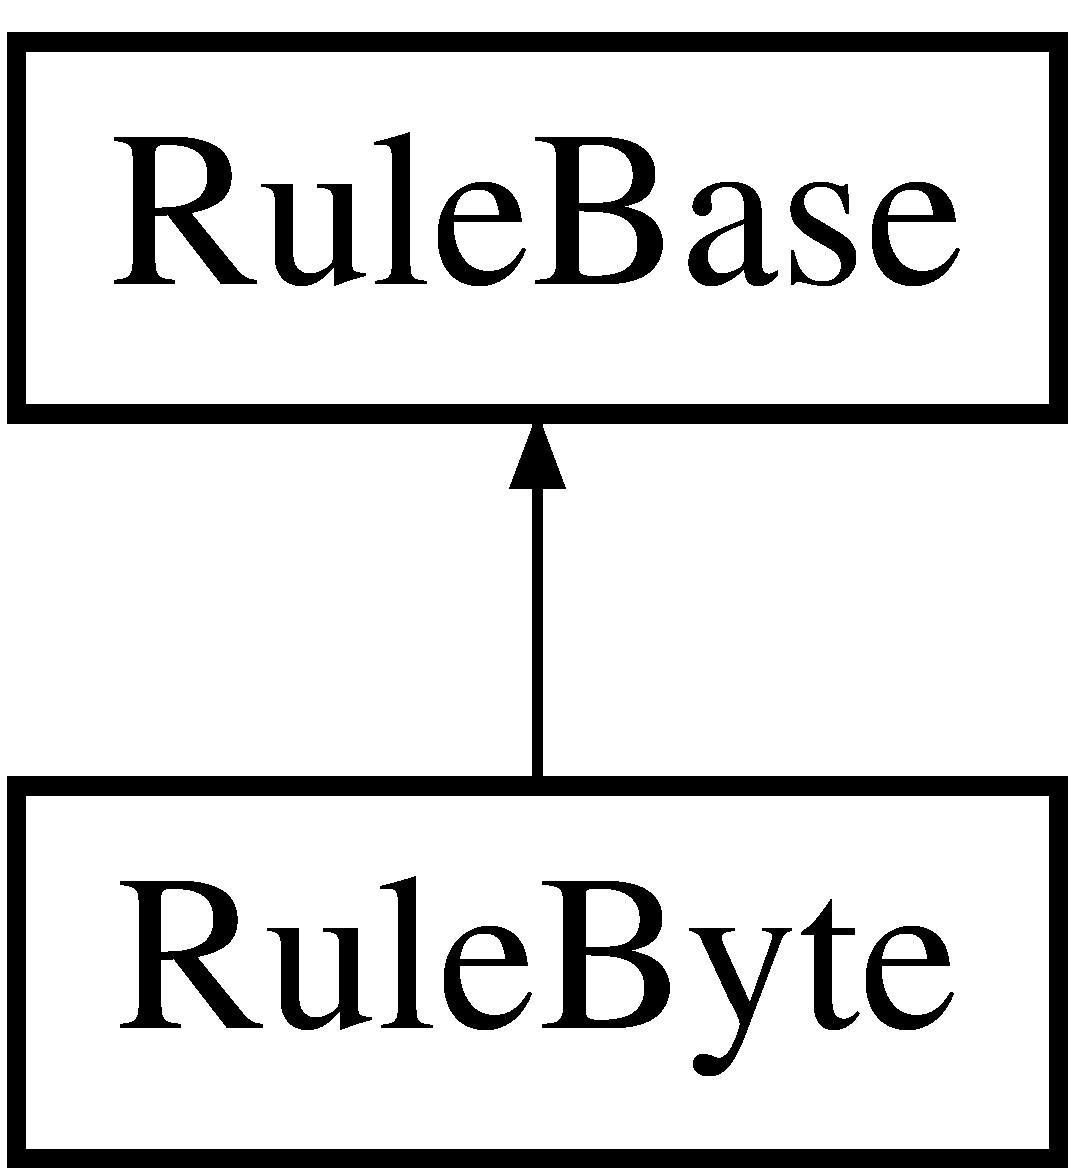
\includegraphics[height=2.000000cm]{class_rule_byte}
\end{center}
\end{figure}
\subsection*{\-Public メソッド}
\begin{DoxyCompactItemize}
\item 
\hyperlink{class_rule_byte_a095c5d389db211932136b53f25f39685}{\-\_\-\-\_\-construct} ()
\item 
\hyperlink{class_rule_byte_afb0fafe7e02a3ae1993c01c19fad2bae}{run} ()
\end{DoxyCompactItemize}


\subsection{説明}
ルール:バイト長クラス

\begin{DoxyVersion}{バージョン}
1.\-0.\-0  \-U\-T\-F-\/8  2011/10/05  2011/10/19 
\end{DoxyVersion}
\begin{DoxyAuthor}{作者}
mamiya\-\_\-shou 
\end{DoxyAuthor}
\begin{DoxyCopyright}{\-Copyright}
mamiya\-\_\-shou  \-M\-I\-T \-License  \-P\-H\-P 5.\-0 以上必須 
\end{DoxyCopyright}


\subsection{コンストラクタとデストラクタ}
\hypertarget{class_rule_byte_a095c5d389db211932136b53f25f39685}{
\index{\-Rule\-Byte@{\-Rule\-Byte}!\-\_\-\-\_\-construct@{\-\_\-\-\_\-construct}}
\index{\-\_\-\-\_\-construct@{\-\_\-\-\_\-construct}!RuleByte@{\-Rule\-Byte}}
\subsubsection[{\-\_\-\-\_\-construct}]{\setlength{\rightskip}{0pt plus 5cm}\-\_\-\-\_\-construct (
\begin{DoxyParamCaption}
{}
\end{DoxyParamCaption}
)}}
\label{class_rule_byte_a095c5d389db211932136b53f25f39685}
コンストラクタ

public \begin{DoxyReturn}{戻り値}
void 
\end{DoxyReturn}


\subsection{関数}
\hypertarget{class_rule_byte_afb0fafe7e02a3ae1993c01c19fad2bae}{
\index{\-Rule\-Byte@{\-Rule\-Byte}!run@{run}}
\index{run@{run}!RuleByte@{\-Rule\-Byte}}
\subsubsection[{run}]{\setlength{\rightskip}{0pt plus 5cm}run (
\begin{DoxyParamCaption}
{}
\end{DoxyParamCaption}
)}}
\label{class_rule_byte_afb0fafe7e02a3ae1993c01c19fad2bae}
バリデートする

public \begin{DoxyReturn}{戻り値}
boolean \-T\-R\-U\-E(\-O\-K) / string エラーメッセージ(\-N\-G) 
\end{DoxyReturn}

\begin{DoxyExceptions}{例外}
{\em \-Exception} & \hyperlink{validate_8php}{validate.\-php} \hyperlink{class_rule_byte_afb0fafe7e02a3ae1993c01c19fad2bae}{run()}で捕捉する  未入力('')の場合は\-T\-R\-U\-Eを返す \\
\hline
\end{DoxyExceptions}


\hyperlink{class_rule_base_afb0fafe7e02a3ae1993c01c19fad2bae}{\-Rule\-Base}を再定義しています。



このクラスの説明は次のファイルから生成されました\-:\begin{DoxyCompactItemize}
\item 
rules/\hyperlink{byte_8php}{byte.\-php}\end{DoxyCompactItemize}

\hypertarget{class_rule_comparison}{\section{Rule\+Comparison クラス}
\label{class_rule_comparison}\index{Rule\+Comparison@{Rule\+Comparison}}
}
Rule\+Comparison の継承関係図\begin{figure}[H]
\begin{center}
\leavevmode
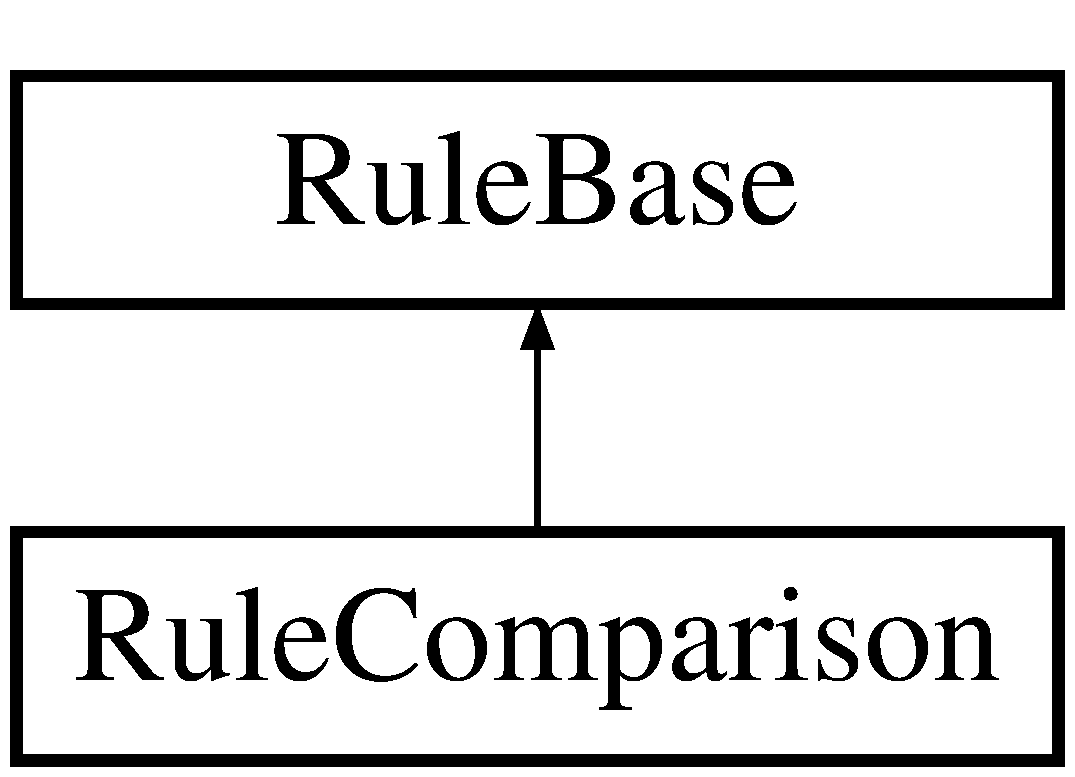
\includegraphics[height=2.000000cm]{class_rule_comparison}
\end{center}
\end{figure}
\subsection*{公開メンバ関数}
\begin{DoxyCompactItemize}
\item 
\hyperlink{class_rule_comparison_a095c5d389db211932136b53f25f39685}{\+\_\+\+\_\+construct} ()
\item 
\hyperlink{class_rule_comparison_afb0fafe7e02a3ae1993c01c19fad2bae}{run} ()
\end{DoxyCompactItemize}
\subsection*{その他の継承メンバ}


\subsection{詳解}
ルール:比較クラス

\begin{DoxyVersion}{バージョン}
1.\+0.\+0  U\+T\+F-\/8  2011/10/19  2011/10/19 
\end{DoxyVersion}
\begin{DoxyAuthor}{著者}
mamiya\+\_\+shou 
\end{DoxyAuthor}
\begin{DoxyCopyright}{著作権所有}
mamiya\+\_\+shou  M\+I\+T License  P\+H\+P 5.\+0 以上必須 
\end{DoxyCopyright}


\subsection{構築子と解体子}
\hypertarget{class_rule_comparison_a095c5d389db211932136b53f25f39685}{\index{Rule\+Comparison@{Rule\+Comparison}!\+\_\+\+\_\+construct@{\+\_\+\+\_\+construct}}
\index{\+\_\+\+\_\+construct@{\+\_\+\+\_\+construct}!Rule\+Comparison@{Rule\+Comparison}}
\subsubsection[{\+\_\+\+\_\+construct}]{\setlength{\rightskip}{0pt plus 5cm}\+\_\+\+\_\+construct (
\begin{DoxyParamCaption}
{}
\end{DoxyParamCaption}
)}}\label{class_rule_comparison_a095c5d389db211932136b53f25f39685}
コンストラクタ

public \begin{DoxyReturn}{戻り値}
void 
\end{DoxyReturn}


\subsection{関数詳解}
\hypertarget{class_rule_comparison_afb0fafe7e02a3ae1993c01c19fad2bae}{\index{Rule\+Comparison@{Rule\+Comparison}!run@{run}}
\index{run@{run}!Rule\+Comparison@{Rule\+Comparison}}
\subsubsection[{run}]{\setlength{\rightskip}{0pt plus 5cm}run (
\begin{DoxyParamCaption}
{}
\end{DoxyParamCaption}
)}}\label{class_rule_comparison_afb0fafe7e02a3ae1993c01c19fad2bae}
バリデートする

public \begin{DoxyReturn}{戻り値}
boolean T\+R\+U\+E(\+O\+K) / string エラーメッセージ(\+N\+G) 
\end{DoxyReturn}

\begin{DoxyExceptions}{例外}
{\em Exception} & validate.\+php \hyperlink{class_rule_comparison_afb0fafe7e02a3ae1993c01c19fad2bae}{run()}で捕捉する  全て未入力('')の場合は\+T\+R\+U\+Eを返す \\
\hline
\end{DoxyExceptions}


このクラス詳解は次のファイルから抽出されました\+:\begin{DoxyCompactItemize}
\item 
Validate/rules/comparison.\+php\end{DoxyCompactItemize}

\hypertarget{class_rule_credit}{\section{Rule\+Credit クラス}
\label{class_rule_credit}\index{Rule\+Credit@{Rule\+Credit}}
}
Rule\+Credit の継承関係図\begin{figure}[H]
\begin{center}
\leavevmode
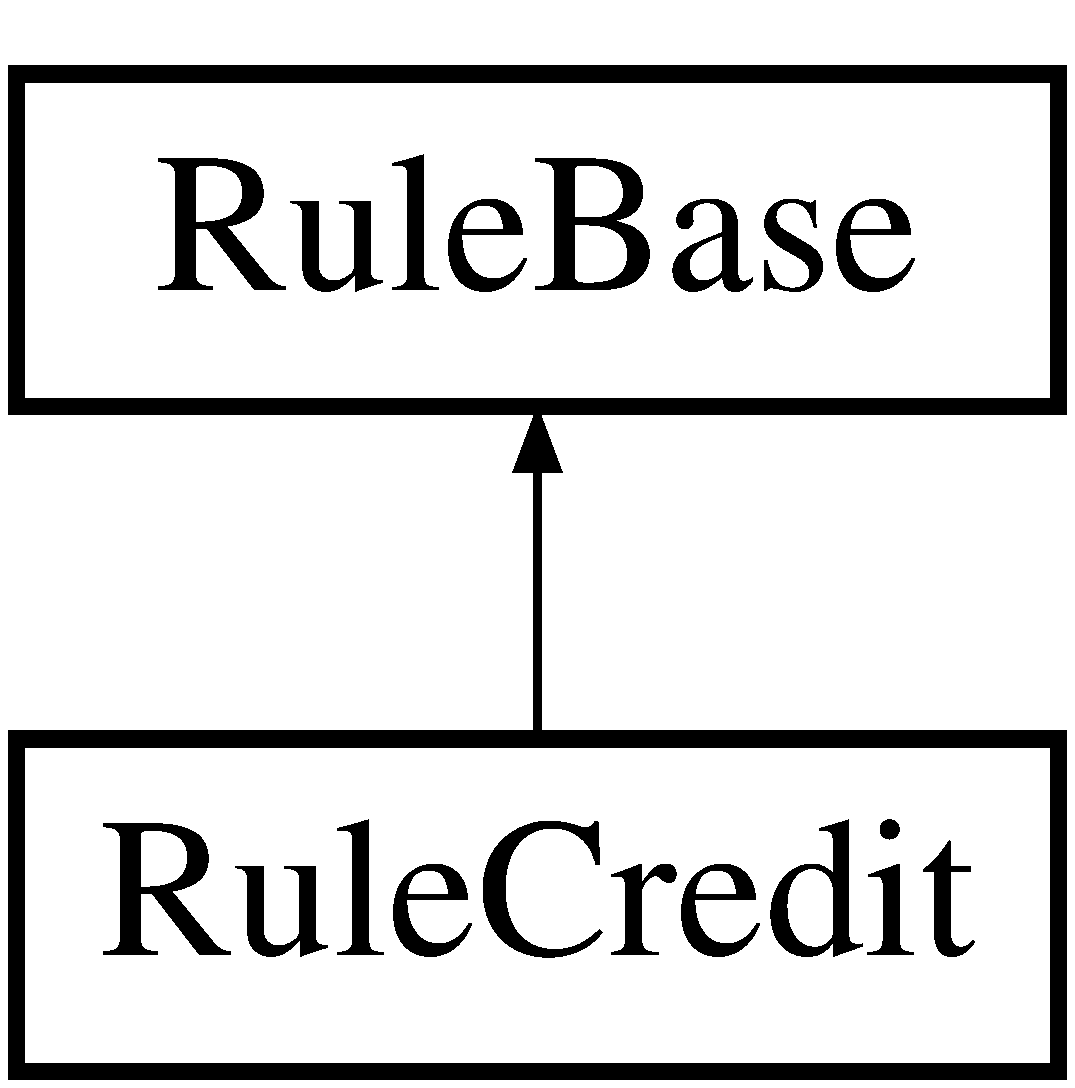
\includegraphics[height=2.000000cm]{class_rule_credit}
\end{center}
\end{figure}
\subsection*{公開メンバ関数}
\begin{DoxyCompactItemize}
\item 
\hyperlink{class_rule_credit_a095c5d389db211932136b53f25f39685}{\+\_\+\+\_\+construct} ()
\item 
\hyperlink{class_rule_credit_afb0fafe7e02a3ae1993c01c19fad2bae}{run} ()
\end{DoxyCompactItemize}
\subsection*{その他の継承メンバ}


\subsection{詳解}
ルール:クレジットカード番号クラス

\begin{DoxyVersion}{バージョン}
1.\+0.\+0  U\+T\+F-\/8  2011/10/10  2011/10/19 
\end{DoxyVersion}
\begin{DoxyAuthor}{著者}
mamiya\+\_\+shou 
\end{DoxyAuthor}
\begin{DoxyCopyright}{著作権所有}
mamiya\+\_\+shou  M\+I\+T License  P\+H\+P 5.\+0 以上必須 
\end{DoxyCopyright}


\subsection{構築子と解体子}
\hypertarget{class_rule_credit_a095c5d389db211932136b53f25f39685}{\index{Rule\+Credit@{Rule\+Credit}!\+\_\+\+\_\+construct@{\+\_\+\+\_\+construct}}
\index{\+\_\+\+\_\+construct@{\+\_\+\+\_\+construct}!Rule\+Credit@{Rule\+Credit}}
\subsubsection[{\+\_\+\+\_\+construct}]{\setlength{\rightskip}{0pt plus 5cm}\+\_\+\+\_\+construct (
\begin{DoxyParamCaption}
{}
\end{DoxyParamCaption}
)}}\label{class_rule_credit_a095c5d389db211932136b53f25f39685}
コンストラクタ

public \begin{DoxyReturn}{戻り値}
void 
\end{DoxyReturn}


\subsection{関数詳解}
\hypertarget{class_rule_credit_afb0fafe7e02a3ae1993c01c19fad2bae}{\index{Rule\+Credit@{Rule\+Credit}!run@{run}}
\index{run@{run}!Rule\+Credit@{Rule\+Credit}}
\subsubsection[{run}]{\setlength{\rightskip}{0pt plus 5cm}run (
\begin{DoxyParamCaption}
{}
\end{DoxyParamCaption}
)}}\label{class_rule_credit_afb0fafe7e02a3ae1993c01c19fad2bae}
バリデートする

public \begin{DoxyReturn}{戻り値}
boolean T\+R\+U\+E(\+O\+K) / string エラーメッセージ(\+N\+G)  未入力('')の場合は\+T\+R\+U\+Eを返す 
\end{DoxyReturn}


このクラス詳解は次のファイルから抽出されました\+:\begin{DoxyCompactItemize}
\item 
Validate/rules/credit.\+php\end{DoxyCompactItemize}

\hypertarget{class_rule_date}{
\section{クラス \-Rule\-Date}
\label{class_rule_date}\index{\-Rule\-Date@{\-Rule\-Date}}
}
\-Rule\-Dateに対する継承グラフ\begin{figure}[H]
\begin{center}
\leavevmode
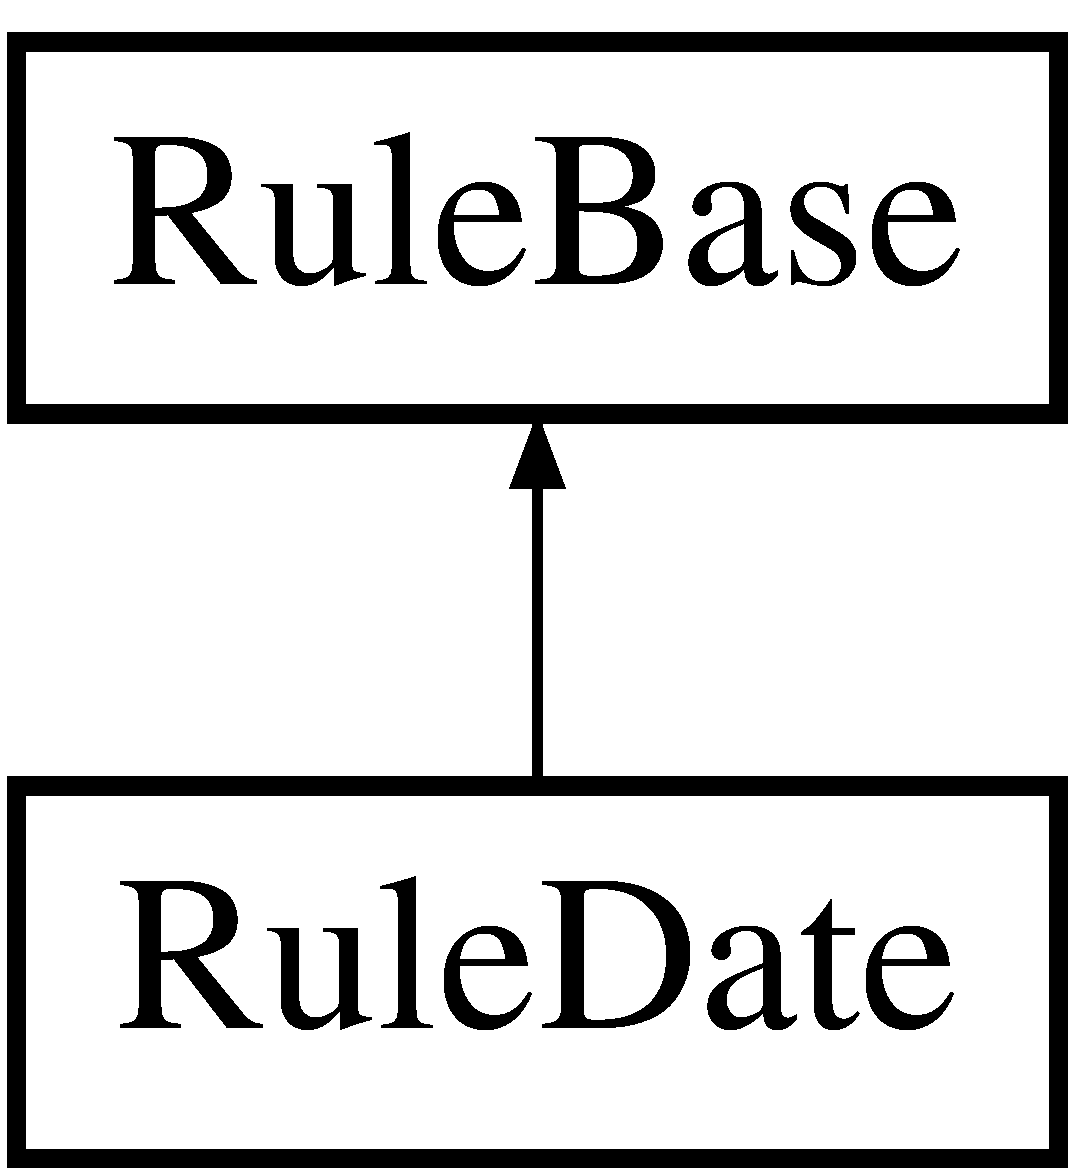
\includegraphics[height=2.000000cm]{class_rule_date}
\end{center}
\end{figure}
\subsection*{\-Public メソッド}
\begin{DoxyCompactItemize}
\item 
\hyperlink{class_rule_date_a095c5d389db211932136b53f25f39685}{\-\_\-\-\_\-construct} ()
\item 
\hyperlink{class_rule_date_afb0fafe7e02a3ae1993c01c19fad2bae}{run} ()
\end{DoxyCompactItemize}


\subsection{説明}
ルール:日付クラス

\begin{DoxyVersion}{バージョン}
1.\-0.\-0  \-U\-T\-F-\/8  2011/10/11  2011/10/19 
\end{DoxyVersion}
\begin{DoxyAuthor}{作者}
mamiya\-\_\-shou 
\end{DoxyAuthor}
\begin{DoxyCopyright}{\-Copyright}
mamiya\-\_\-shou  \-M\-I\-T \-License  \-P\-H\-P 5.\-0 以上必須 
\end{DoxyCopyright}


\subsection{コンストラクタとデストラクタ}
\hypertarget{class_rule_date_a095c5d389db211932136b53f25f39685}{
\index{\-Rule\-Date@{\-Rule\-Date}!\-\_\-\-\_\-construct@{\-\_\-\-\_\-construct}}
\index{\-\_\-\-\_\-construct@{\-\_\-\-\_\-construct}!RuleDate@{\-Rule\-Date}}
\subsubsection[{\-\_\-\-\_\-construct}]{\setlength{\rightskip}{0pt plus 5cm}\-\_\-\-\_\-construct (
\begin{DoxyParamCaption}
{}
\end{DoxyParamCaption}
)}}
\label{class_rule_date_a095c5d389db211932136b53f25f39685}
コンストラクタ

public \begin{DoxyReturn}{戻り値}
void 
\end{DoxyReturn}


\subsection{関数}
\hypertarget{class_rule_date_afb0fafe7e02a3ae1993c01c19fad2bae}{
\index{\-Rule\-Date@{\-Rule\-Date}!run@{run}}
\index{run@{run}!RuleDate@{\-Rule\-Date}}
\subsubsection[{run}]{\setlength{\rightskip}{0pt plus 5cm}run (
\begin{DoxyParamCaption}
{}
\end{DoxyParamCaption}
)}}
\label{class_rule_date_afb0fafe7e02a3ae1993c01c19fad2bae}
バリデートする

public \begin{DoxyReturn}{戻り値}
boolean \-T\-R\-U\-E(\-O\-K) / string エラーメッセージ(\-N\-G) 
\end{DoxyReturn}

\begin{DoxyExceptions}{例外}
{\em \-Exception} & \hyperlink{validate_8php}{validate.\-php} \hyperlink{class_rule_date_afb0fafe7e02a3ae1993c01c19fad2bae}{run()}で捕捉する  未入力('')の場合は\-T\-R\-U\-Eを返す \\
\hline
\end{DoxyExceptions}


\hyperlink{class_rule_base_afb0fafe7e02a3ae1993c01c19fad2bae}{\-Rule\-Base}を再定義しています。



このクラスの説明は次のファイルから生成されました\-:\begin{DoxyCompactItemize}
\item 
rules/\hyperlink{date_8php}{date.\-php}\end{DoxyCompactItemize}

\hypertarget{class_rule_hiragana}{
\section{クラス \-Rule\-Hiragana}
\label{class_rule_hiragana}\index{\-Rule\-Hiragana@{\-Rule\-Hiragana}}
}
\-Rule\-Hiraganaに対する継承グラフ\begin{figure}[H]
\begin{center}
\leavevmode
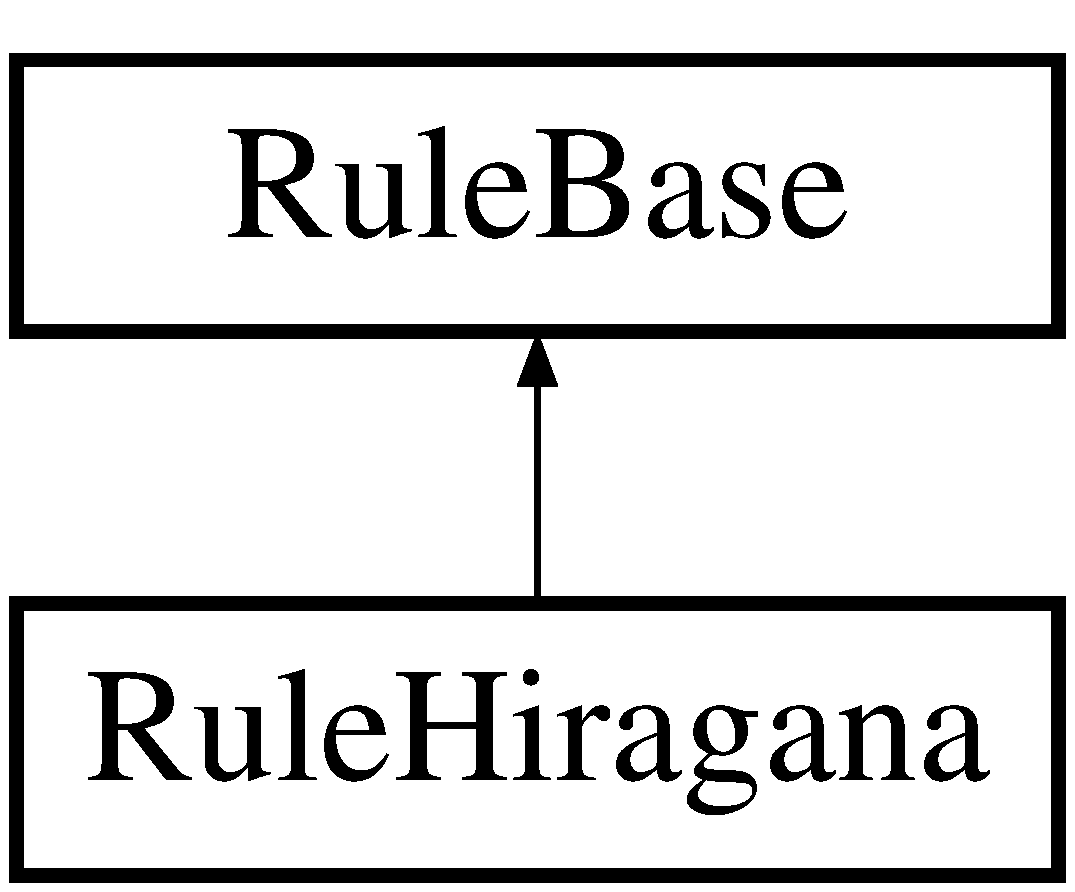
\includegraphics[height=2.000000cm]{class_rule_hiragana}
\end{center}
\end{figure}
\subsection*{\-Public メソッド}
\begin{DoxyCompactItemize}
\item 
\hyperlink{class_rule_hiragana_a095c5d389db211932136b53f25f39685}{\-\_\-\-\_\-construct} ()
\item 
\hyperlink{class_rule_hiragana_afb0fafe7e02a3ae1993c01c19fad2bae}{run} ()
\end{DoxyCompactItemize}


\subsection{説明}
ルール:ひらがなクラス

\begin{DoxyVersion}{バージョン}
1.\-0.\-0  \-U\-T\-F-\/8  2011/10/08  2011/10/19 
\end{DoxyVersion}
\begin{DoxyAuthor}{作者}
mamiya\-\_\-shou 
\end{DoxyAuthor}
\begin{DoxyCopyright}{\-Copyright}
mamiya\-\_\-shou  \-M\-I\-T \-License  \-P\-H\-P 5.\-0 以上必須 
\end{DoxyCopyright}


\subsection{コンストラクタとデストラクタ}
\hypertarget{class_rule_hiragana_a095c5d389db211932136b53f25f39685}{
\index{\-Rule\-Hiragana@{\-Rule\-Hiragana}!\-\_\-\-\_\-construct@{\-\_\-\-\_\-construct}}
\index{\-\_\-\-\_\-construct@{\-\_\-\-\_\-construct}!RuleHiragana@{\-Rule\-Hiragana}}
\subsubsection[{\-\_\-\-\_\-construct}]{\setlength{\rightskip}{0pt plus 5cm}\-\_\-\-\_\-construct (
\begin{DoxyParamCaption}
{}
\end{DoxyParamCaption}
)}}
\label{class_rule_hiragana_a095c5d389db211932136b53f25f39685}
コンストラクタ

public \begin{DoxyReturn}{戻り値}
void 
\end{DoxyReturn}


\subsection{関数}
\hypertarget{class_rule_hiragana_afb0fafe7e02a3ae1993c01c19fad2bae}{
\index{\-Rule\-Hiragana@{\-Rule\-Hiragana}!run@{run}}
\index{run@{run}!RuleHiragana@{\-Rule\-Hiragana}}
\subsubsection[{run}]{\setlength{\rightskip}{0pt plus 5cm}run (
\begin{DoxyParamCaption}
{}
\end{DoxyParamCaption}
)}}
\label{class_rule_hiragana_afb0fafe7e02a3ae1993c01c19fad2bae}
バリデートする

public \begin{DoxyReturn}{戻り値}
boolean \-T\-R\-U\-E(\-O\-K) / string エラーメッセージ(\-N\-G) 
\end{DoxyReturn}

\begin{DoxyExceptions}{例外}
{\em \-Exception} & \hyperlink{validate_8php}{validate.\-php} \hyperlink{class_rule_hiragana_afb0fafe7e02a3ae1993c01c19fad2bae}{run()}で捕捉する  未入力('')の場合は\-T\-R\-U\-Eを返す  » \mbox{[}\-Code\-Igniter\mbox{]} \-Formバリデーションの拡張クラス \-Web \-Sytem $|$ \-A\-I\-D\-R\-E\-A\-M \href{http://blog.aidream.jp/codeigniter/codeigniter-form-validation-extend-class-1351.html}{\tt http\-://blog.\-aidream.\-jp/codeigniter/codeigniter-\/form-\/validation-\/extend-\/class-\/1351.\-html} \\
\hline
\end{DoxyExceptions}


\hyperlink{class_rule_base_afb0fafe7e02a3ae1993c01c19fad2bae}{\-Rule\-Base}を再定義しています。



このクラスの説明は次のファイルから生成されました\-:\begin{DoxyCompactItemize}
\item 
rules/\hyperlink{hiragana_8php}{hiragana.\-php}\end{DoxyCompactItemize}

\hypertarget{class_rule_integer}{
\section{クラス \-Rule\-Integer}
\label{class_rule_integer}\index{\-Rule\-Integer@{\-Rule\-Integer}}
}
\-Rule\-Integerに対する継承グラフ\begin{figure}[H]
\begin{center}
\leavevmode
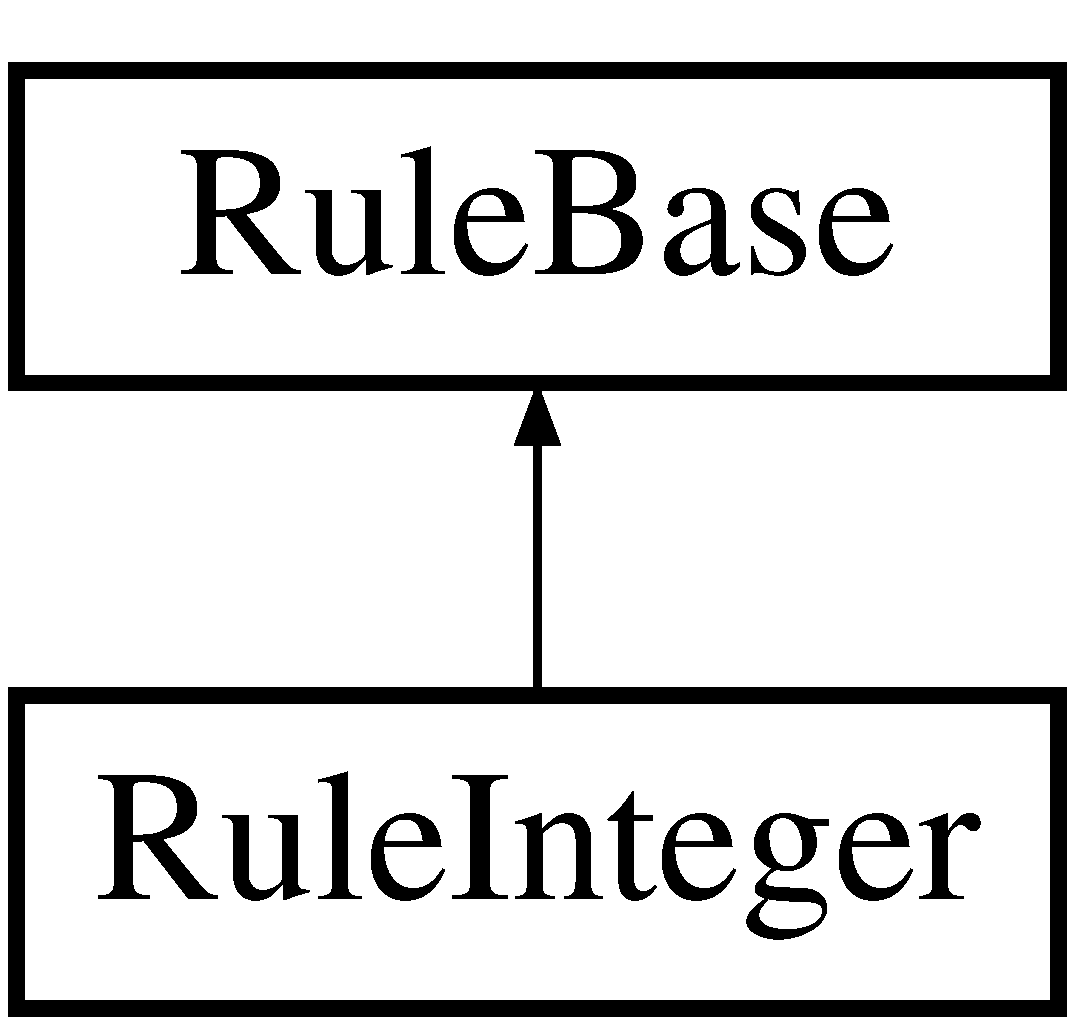
\includegraphics[height=2.000000cm]{class_rule_integer}
\end{center}
\end{figure}
\subsection*{\-Public メソッド}
\begin{DoxyCompactItemize}
\item 
\hyperlink{class_rule_integer_a095c5d389db211932136b53f25f39685}{\-\_\-\-\_\-construct} ()
\item 
\hyperlink{class_rule_integer_afb0fafe7e02a3ae1993c01c19fad2bae}{run} ()
\end{DoxyCompactItemize}


\subsection{説明}
ルール:整数クラス

\begin{DoxyVersion}{バージョン}
1.\-0.\-0  \-U\-T\-F-\/8  2011/10/06  2011/10/19 
\end{DoxyVersion}
\begin{DoxyAuthor}{作者}
mamiya\-\_\-shou 
\end{DoxyAuthor}
\begin{DoxyCopyright}{\-Copyright}
mamiya\-\_\-shou  \-M\-I\-T \-License  \-P\-H\-P 5.\-0 以上必須 
\end{DoxyCopyright}


\subsection{コンストラクタとデストラクタ}
\hypertarget{class_rule_integer_a095c5d389db211932136b53f25f39685}{
\index{\-Rule\-Integer@{\-Rule\-Integer}!\-\_\-\-\_\-construct@{\-\_\-\-\_\-construct}}
\index{\-\_\-\-\_\-construct@{\-\_\-\-\_\-construct}!RuleInteger@{\-Rule\-Integer}}
\subsubsection[{\-\_\-\-\_\-construct}]{\setlength{\rightskip}{0pt plus 5cm}\-\_\-\-\_\-construct (
\begin{DoxyParamCaption}
{}
\end{DoxyParamCaption}
)}}
\label{class_rule_integer_a095c5d389db211932136b53f25f39685}
コンストラクタ

public \begin{DoxyReturn}{戻り値}
void 
\end{DoxyReturn}


\subsection{関数}
\hypertarget{class_rule_integer_afb0fafe7e02a3ae1993c01c19fad2bae}{
\index{\-Rule\-Integer@{\-Rule\-Integer}!run@{run}}
\index{run@{run}!RuleInteger@{\-Rule\-Integer}}
\subsubsection[{run}]{\setlength{\rightskip}{0pt plus 5cm}run (
\begin{DoxyParamCaption}
{}
\end{DoxyParamCaption}
)}}
\label{class_rule_integer_afb0fafe7e02a3ae1993c01c19fad2bae}
バリデートする

public \begin{DoxyReturn}{戻り値}
boolean \-T\-R\-U\-E(\-O\-K) / string エラーメッセージ(\-N\-G)  未入力('')の場合は\-T\-R\-U\-Eを返す 
\end{DoxyReturn}


\hyperlink{class_rule_base_afb0fafe7e02a3ae1993c01c19fad2bae}{\-Rule\-Base}を再定義しています。



このクラスの説明は次のファイルから生成されました\-:\begin{DoxyCompactItemize}
\item 
rules/\hyperlink{integer_8php}{integer.\-php}\end{DoxyCompactItemize}

\hypertarget{class_rule_katakana}{\section{Rule\+Katakana クラス}
\label{class_rule_katakana}\index{Rule\+Katakana@{Rule\+Katakana}}
}
Rule\+Katakana の継承関係図\begin{figure}[H]
\begin{center}
\leavevmode
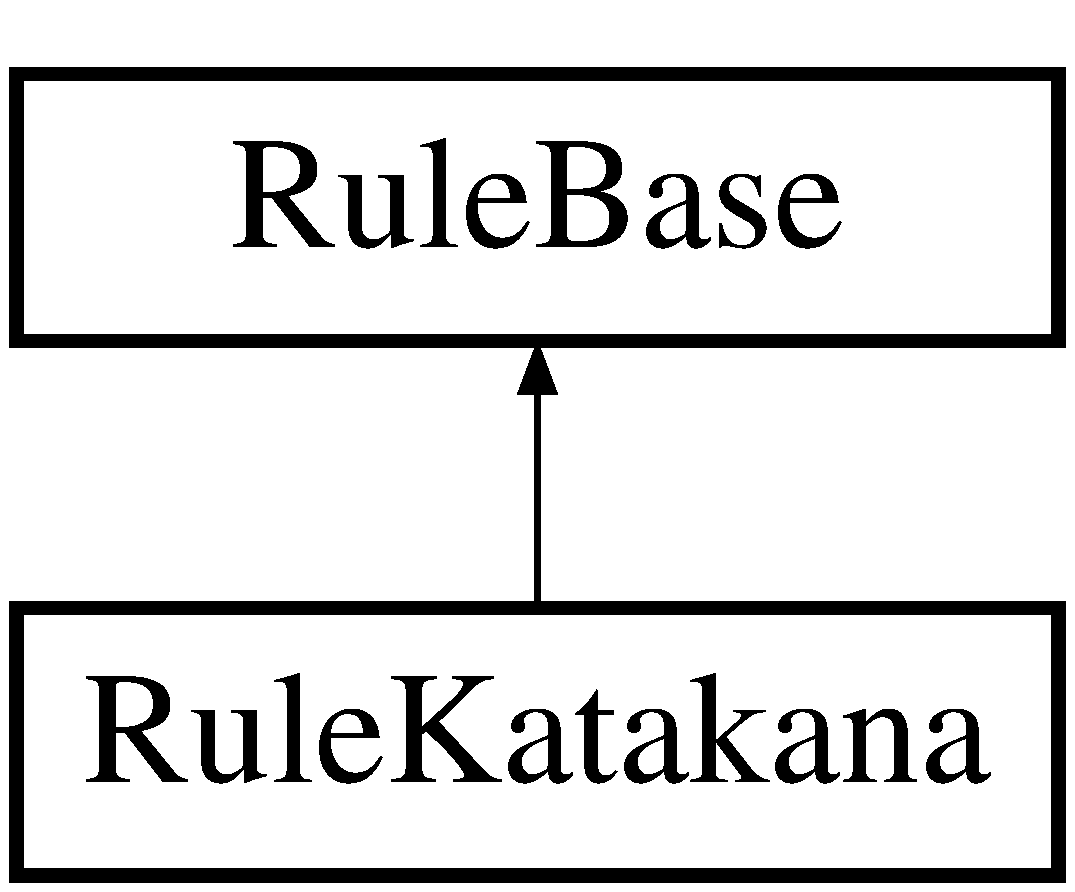
\includegraphics[height=2.000000cm]{class_rule_katakana}
\end{center}
\end{figure}
\subsection*{公開メンバ関数}
\begin{DoxyCompactItemize}
\item 
\hyperlink{class_rule_katakana_a095c5d389db211932136b53f25f39685}{\+\_\+\+\_\+construct} ()
\item 
\hyperlink{class_rule_katakana_afb0fafe7e02a3ae1993c01c19fad2bae}{run} ()
\end{DoxyCompactItemize}
\subsection*{その他の継承メンバ}


\subsection{詳解}
ルール:カタカナクラス

\begin{DoxyVersion}{バージョン}
1.\+0.\+0  U\+T\+F-\/8  2011/10/09  2011/10/19 
\end{DoxyVersion}
\begin{DoxyAuthor}{著者}
mamiya\+\_\+shou 
\end{DoxyAuthor}
\begin{DoxyCopyright}{著作権所有}
mamiya\+\_\+shou  M\+I\+T License  P\+H\+P 5.\+0 以上必須 
\end{DoxyCopyright}


\subsection{構築子と解体子}
\hypertarget{class_rule_katakana_a095c5d389db211932136b53f25f39685}{\index{Rule\+Katakana@{Rule\+Katakana}!\+\_\+\+\_\+construct@{\+\_\+\+\_\+construct}}
\index{\+\_\+\+\_\+construct@{\+\_\+\+\_\+construct}!Rule\+Katakana@{Rule\+Katakana}}
\subsubsection[{\+\_\+\+\_\+construct}]{\setlength{\rightskip}{0pt plus 5cm}\+\_\+\+\_\+construct (
\begin{DoxyParamCaption}
{}
\end{DoxyParamCaption}
)}}\label{class_rule_katakana_a095c5d389db211932136b53f25f39685}
コンストラクタ

public \begin{DoxyReturn}{戻り値}
void 
\end{DoxyReturn}


\subsection{関数詳解}
\hypertarget{class_rule_katakana_afb0fafe7e02a3ae1993c01c19fad2bae}{\index{Rule\+Katakana@{Rule\+Katakana}!run@{run}}
\index{run@{run}!Rule\+Katakana@{Rule\+Katakana}}
\subsubsection[{run}]{\setlength{\rightskip}{0pt plus 5cm}run (
\begin{DoxyParamCaption}
{}
\end{DoxyParamCaption}
)}}\label{class_rule_katakana_afb0fafe7e02a3ae1993c01c19fad2bae}
バリデートする

public \begin{DoxyReturn}{戻り値}
boolean T\+R\+U\+E(\+O\+K) / string エラーメッセージ(\+N\+G) 
\end{DoxyReturn}

\begin{DoxyExceptions}{例外}
{\em Exception} & validate.\+php \hyperlink{class_rule_katakana_afb0fafe7e02a3ae1993c01c19fad2bae}{run()}で捕捉する  未入力('')の場合は\+T\+R\+U\+Eを返す  » \mbox{[}Code\+Igniter\mbox{]} Formバリデーションの拡張クラス Web Sytem $\vert$ A\+I\+D\+R\+E\+A\+M \href{http://blog.aidream.jp/codeigniter/codeigniter-form-validation-extend-class-1351.html}{\tt http\+://blog.\+aidream.\+jp/codeigniter/codeigniter-\/form-\/validation-\/extend-\/class-\/1351.\+html} \\
\hline
\end{DoxyExceptions}


このクラス詳解は次のファイルから抽出されました\+:\begin{DoxyCompactItemize}
\item 
Validate/rules/katakana.\+php\end{DoxyCompactItemize}

\hypertarget{class_rule_length}{
\section{クラス \-Rule\-Length}
\label{class_rule_length}\index{\-Rule\-Length@{\-Rule\-Length}}
}
\-Rule\-Lengthに対する継承グラフ\begin{figure}[H]
\begin{center}
\leavevmode
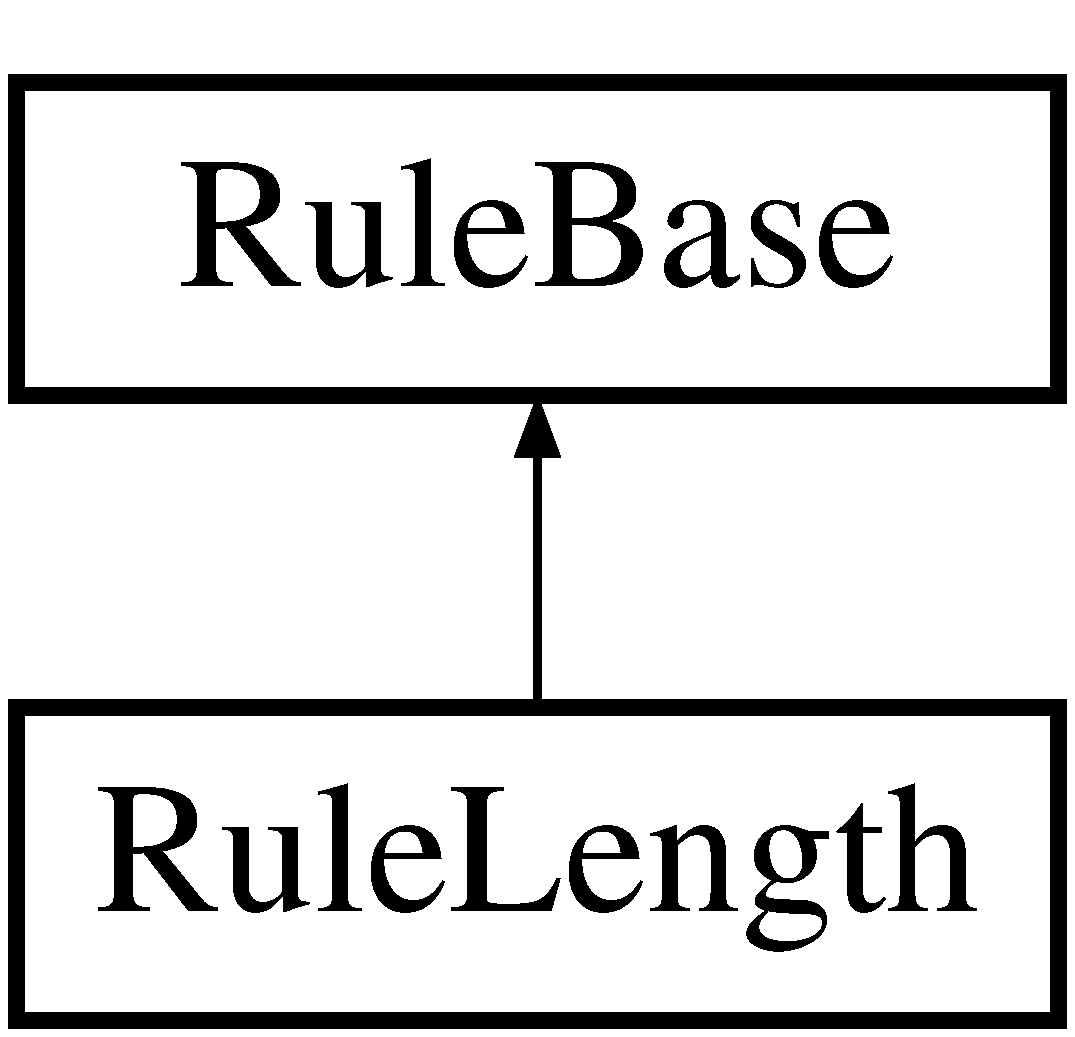
\includegraphics[height=2.000000cm]{class_rule_length}
\end{center}
\end{figure}
\subsection*{\-Public メソッド}
\begin{DoxyCompactItemize}
\item 
\hyperlink{class_rule_length_a095c5d389db211932136b53f25f39685}{\-\_\-\-\_\-construct} ()
\item 
\hyperlink{class_rule_length_afb0fafe7e02a3ae1993c01c19fad2bae}{run} ()
\end{DoxyCompactItemize}


\subsection{説明}
ルール:文字長クラス

\begin{DoxyVersion}{バージョン}
1.\-0.\-0  \-U\-T\-F-\/8  2011/10/05  2011/10/19 
\end{DoxyVersion}
\begin{DoxyAuthor}{作者}
mamiya\-\_\-shou 
\end{DoxyAuthor}
\begin{DoxyCopyright}{\-Copyright}
mamiya\-\_\-shou  \-M\-I\-T \-License 
\end{DoxyCopyright}


\subsection{コンストラクタとデストラクタ}
\hypertarget{class_rule_length_a095c5d389db211932136b53f25f39685}{
\index{\-Rule\-Length@{\-Rule\-Length}!\-\_\-\-\_\-construct@{\-\_\-\-\_\-construct}}
\index{\-\_\-\-\_\-construct@{\-\_\-\-\_\-construct}!RuleLength@{\-Rule\-Length}}
\subsubsection[{\-\_\-\-\_\-construct}]{\setlength{\rightskip}{0pt plus 5cm}\-\_\-\-\_\-construct (
\begin{DoxyParamCaption}
{}
\end{DoxyParamCaption}
)}}
\label{class_rule_length_a095c5d389db211932136b53f25f39685}
コンストラクタ

public \begin{DoxyReturn}{戻り値}
void 
\end{DoxyReturn}


\subsection{関数}
\hypertarget{class_rule_length_afb0fafe7e02a3ae1993c01c19fad2bae}{
\index{\-Rule\-Length@{\-Rule\-Length}!run@{run}}
\index{run@{run}!RuleLength@{\-Rule\-Length}}
\subsubsection[{run}]{\setlength{\rightskip}{0pt plus 5cm}run (
\begin{DoxyParamCaption}
{}
\end{DoxyParamCaption}
)}}
\label{class_rule_length_afb0fafe7e02a3ae1993c01c19fad2bae}
バリデートする

public \begin{DoxyReturn}{戻り値}
boolean \-T\-R\-U\-E(\-O\-K) / string エラーメッセージ(\-N\-G) 
\end{DoxyReturn}

\begin{DoxyExceptions}{例外}
{\em \-Exception} & \hyperlink{validate_8php}{validate.\-php} \hyperlink{class_rule_length_afb0fafe7e02a3ae1993c01c19fad2bae}{run()}で捕捉する  未入力('')の場合は\-T\-R\-U\-Eを返す \\
\hline
\end{DoxyExceptions}


\hyperlink{class_rule_base_afb0fafe7e02a3ae1993c01c19fad2bae}{\-Rule\-Base}を再定義しています。



このクラスの説明は次のファイルから生成されました\-:\begin{DoxyCompactItemize}
\item 
rules/\hyperlink{length_8php}{length.\-php}\end{DoxyCompactItemize}

\hypertarget{class_rule_mail}{
\section{クラス \-Rule\-Mail}
\label{class_rule_mail}\index{\-Rule\-Mail@{\-Rule\-Mail}}
}
\-Rule\-Mailに対する継承グラフ\begin{figure}[H]
\begin{center}
\leavevmode
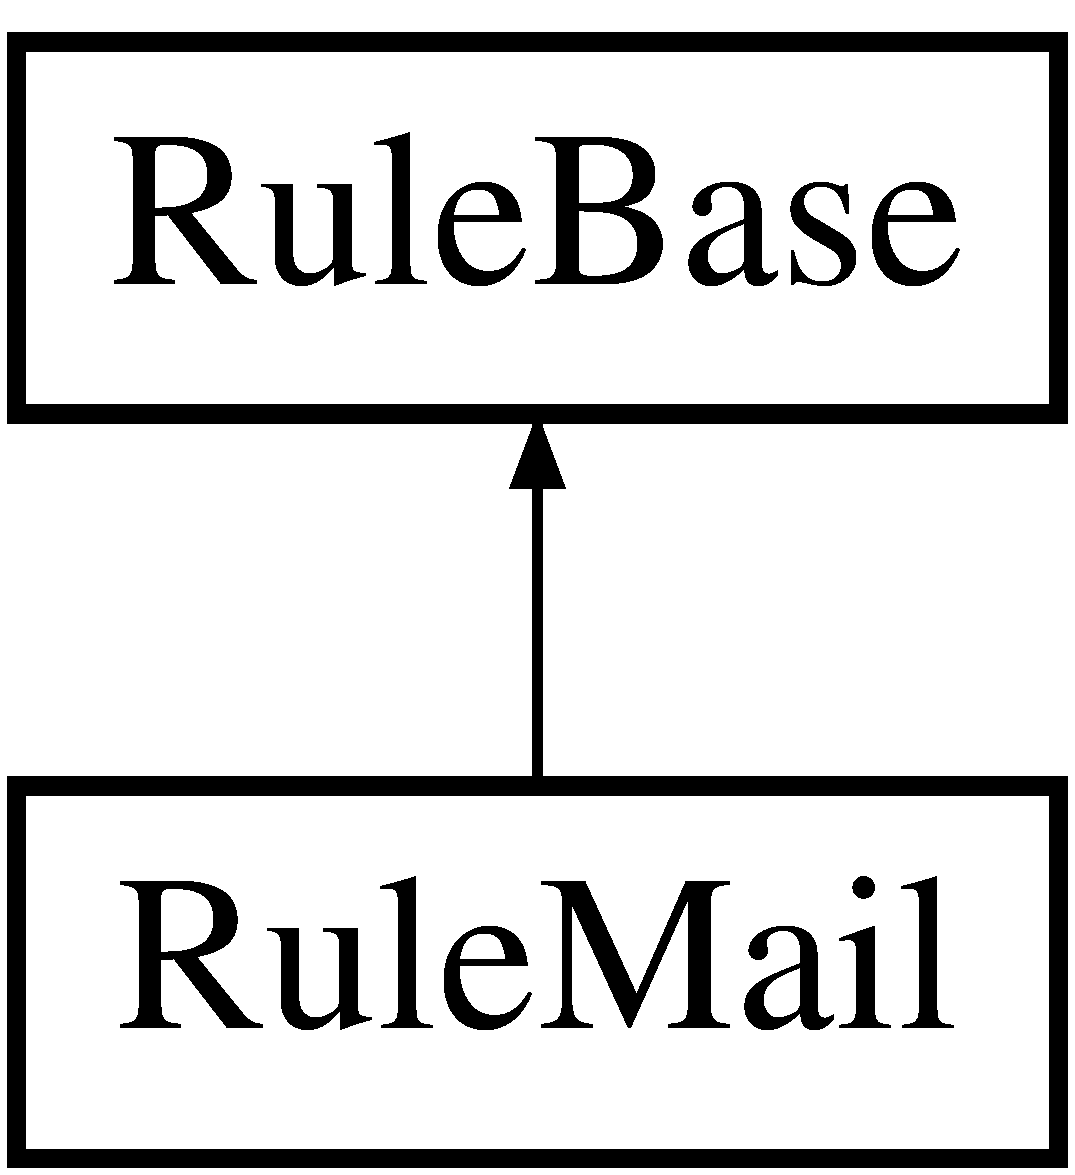
\includegraphics[height=2.000000cm]{class_rule_mail}
\end{center}
\end{figure}
\subsection*{\-Public メソッド}
\begin{DoxyCompactItemize}
\item 
\hyperlink{class_rule_mail_a095c5d389db211932136b53f25f39685}{\-\_\-\-\_\-construct} ()
\item 
\hyperlink{class_rule_mail_afb0fafe7e02a3ae1993c01c19fad2bae}{run} ()
\end{DoxyCompactItemize}
\subsection*{変数}
\begin{DoxyCompactItemize}
\item 
const \hyperlink{class_rule_mail_ae120b9206d39e1922b268a74697c4775}{\-M\-A\-I\-L\-\_\-\-P\-A\-T\-T\-E\-R\-N} = '/$^\wedge$(\mbox{[}a-\/z0-\/9\-\_\-\mbox{]}$|$$\backslash$-\/$|$$\backslash$.$|$$\backslash$+)+@((\mbox{[}a-\/z0-\/9\-\_\-\mbox{]}$|$$\backslash$-\/)+$\backslash$.)+\mbox{[}a-\/z\mbox{]}\{2,6\}\$/i'
\end{DoxyCompactItemize}


\subsection{説明}
ルール:メールアドレスクラス

\begin{DoxyVersion}{バージョン}
1.\-0.\-0  \-U\-T\-F-\/8  2011/10/09  2011/10/19 
\end{DoxyVersion}
\begin{DoxyAuthor}{作者}
mamiya\-\_\-shou 
\end{DoxyAuthor}
\begin{DoxyCopyright}{\-Copyright}
mamiya\-\_\-shou  \-M\-I\-T \-License  \-P\-H\-P 5.\-0 以上必須 
\end{DoxyCopyright}


\subsection{コンストラクタとデストラクタ}
\hypertarget{class_rule_mail_a095c5d389db211932136b53f25f39685}{
\index{\-Rule\-Mail@{\-Rule\-Mail}!\-\_\-\-\_\-construct@{\-\_\-\-\_\-construct}}
\index{\-\_\-\-\_\-construct@{\-\_\-\-\_\-construct}!RuleMail@{\-Rule\-Mail}}
\subsubsection[{\-\_\-\-\_\-construct}]{\setlength{\rightskip}{0pt plus 5cm}\-\_\-\-\_\-construct (
\begin{DoxyParamCaption}
{}
\end{DoxyParamCaption}
)}}
\label{class_rule_mail_a095c5d389db211932136b53f25f39685}
コンストラクタ

public \begin{DoxyReturn}{戻り値}
void 
\end{DoxyReturn}


\subsection{関数}
\hypertarget{class_rule_mail_afb0fafe7e02a3ae1993c01c19fad2bae}{
\index{\-Rule\-Mail@{\-Rule\-Mail}!run@{run}}
\index{run@{run}!RuleMail@{\-Rule\-Mail}}
\subsubsection[{run}]{\setlength{\rightskip}{0pt plus 5cm}run (
\begin{DoxyParamCaption}
{}
\end{DoxyParamCaption}
)}}
\label{class_rule_mail_afb0fafe7e02a3ae1993c01c19fad2bae}
バリデートする

public \begin{DoxyReturn}{戻り値}
boolean \-T\-R\-U\-E(\-O\-K) / string エラーメッセージ(\-N\-G)  未入力('')の場合は\-T\-R\-U\-Eを返す  re\-: \-P\-H\-Pでメールアドレスかどうか調べる方法 (ハズレ日記) \href{http://catbot.net/blog/2007/06/re_php.html}{\tt http\-://catbot.\-net/blog/2007/06/re\-\_\-php.\-html} 
\end{DoxyReturn}


\hyperlink{class_rule_base_afb0fafe7e02a3ae1993c01c19fad2bae}{\-Rule\-Base}を再定義しています。



\subsection{構造体}
\hypertarget{class_rule_mail_ae120b9206d39e1922b268a74697c4775}{
\index{\-Rule\-Mail@{\-Rule\-Mail}!\-M\-A\-I\-L\-\_\-\-P\-A\-T\-T\-E\-R\-N@{\-M\-A\-I\-L\-\_\-\-P\-A\-T\-T\-E\-R\-N}}
\index{\-M\-A\-I\-L\-\_\-\-P\-A\-T\-T\-E\-R\-N@{\-M\-A\-I\-L\-\_\-\-P\-A\-T\-T\-E\-R\-N}!RuleMail@{\-Rule\-Mail}}
\subsubsection[{\-M\-A\-I\-L\-\_\-\-P\-A\-T\-T\-E\-R\-N}]{\setlength{\rightskip}{0pt plus 5cm}const {\bf \-M\-A\-I\-L\-\_\-\-P\-A\-T\-T\-E\-R\-N} = '/$^\wedge$(\mbox{[}a-\/z0-\/9\-\_\-\mbox{]}$|$$\backslash$-\/$|$$\backslash$.$|$$\backslash$+)+@((\mbox{[}a-\/z0-\/9\-\_\-\mbox{]}$|$$\backslash$-\/)+$\backslash$.)+\mbox{[}a-\/z\mbox{]}\{2,6\}\$/i'}}
\label{class_rule_mail_ae120b9206d39e1922b268a74697c4775}


このクラスの説明は次のファイルから生成されました\-:\begin{DoxyCompactItemize}
\item 
rules/\hyperlink{mail_8php}{mail.\-php}\end{DoxyCompactItemize}

\hypertarget{class_rule_multi}{
\section{クラス \-Rule\-Multi}
\label{class_rule_multi}\index{\-Rule\-Multi@{\-Rule\-Multi}}
}
\-Rule\-Multiに対する継承グラフ\begin{figure}[H]
\begin{center}
\leavevmode
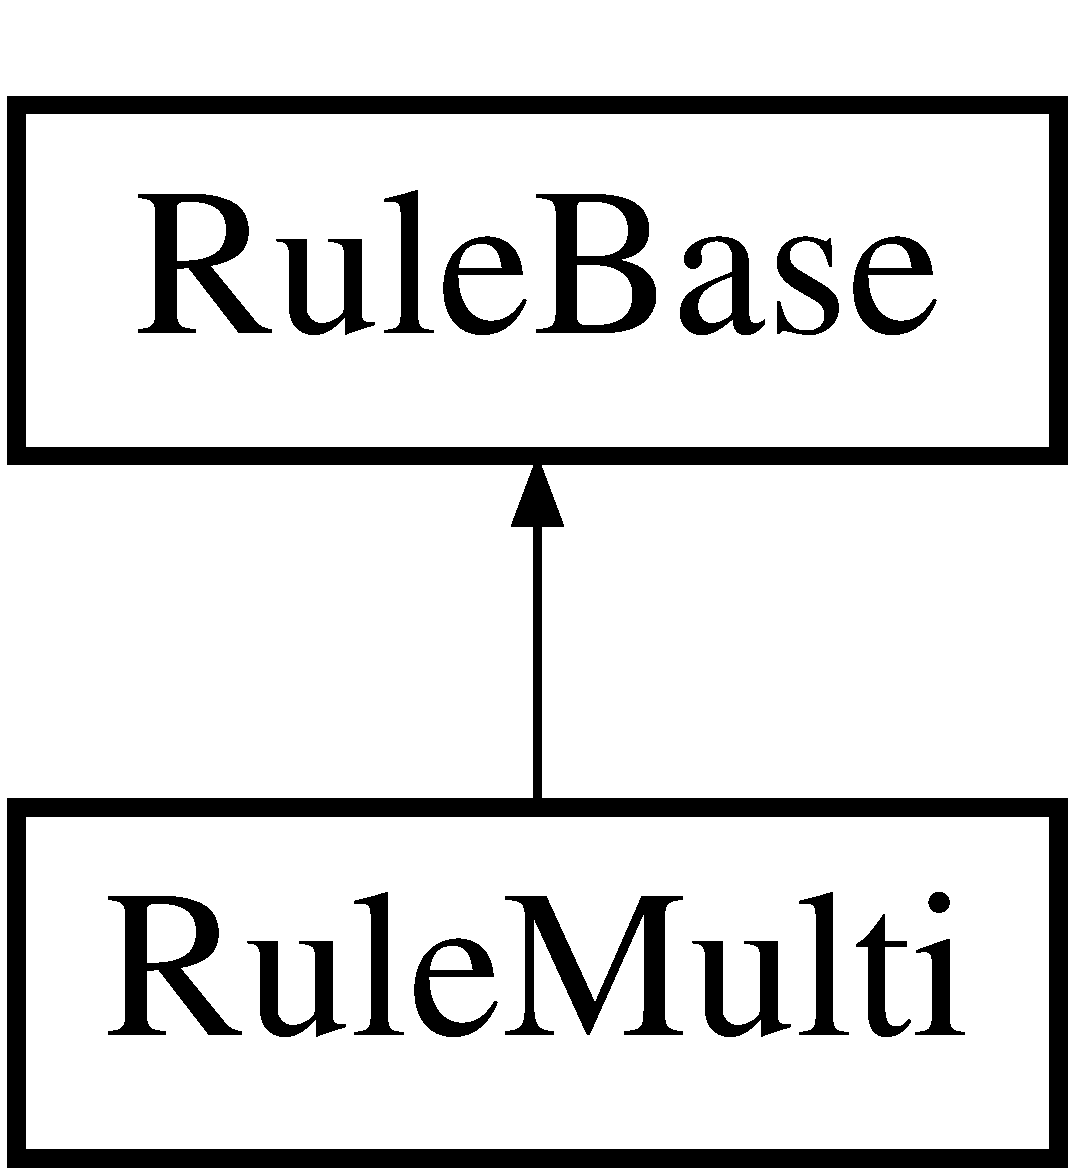
\includegraphics[height=2.000000cm]{class_rule_multi}
\end{center}
\end{figure}
\subsection*{\-Public メソッド}
\begin{DoxyCompactItemize}
\item 
\hyperlink{class_rule_multi_a095c5d389db211932136b53f25f39685}{\-\_\-\-\_\-construct} ()
\item 
\hyperlink{class_rule_multi_afb0fafe7e02a3ae1993c01c19fad2bae}{run} ()
\end{DoxyCompactItemize}


\subsection{説明}
ルール:全角文字クラス

\begin{DoxyVersion}{バージョン}
1.\-0.\-0  \-U\-T\-F-\/8  2011/10/08  2011/10/19 
\end{DoxyVersion}
\begin{DoxyAuthor}{作者}
mamiya\-\_\-shou 
\end{DoxyAuthor}
\begin{DoxyCopyright}{\-Copyright}
mamiya\-\_\-shou  \-M\-I\-T \-License  \-P\-H\-P 5.\-0 以上必須 
\end{DoxyCopyright}


\subsection{コンストラクタとデストラクタ}
\hypertarget{class_rule_multi_a095c5d389db211932136b53f25f39685}{
\index{\-Rule\-Multi@{\-Rule\-Multi}!\-\_\-\-\_\-construct@{\-\_\-\-\_\-construct}}
\index{\-\_\-\-\_\-construct@{\-\_\-\-\_\-construct}!RuleMulti@{\-Rule\-Multi}}
\subsubsection[{\-\_\-\-\_\-construct}]{\setlength{\rightskip}{0pt plus 5cm}\-\_\-\-\_\-construct (
\begin{DoxyParamCaption}
{}
\end{DoxyParamCaption}
)}}
\label{class_rule_multi_a095c5d389db211932136b53f25f39685}
コンストラクタ

public \begin{DoxyReturn}{戻り値}
void 
\end{DoxyReturn}


\subsection{関数}
\hypertarget{class_rule_multi_afb0fafe7e02a3ae1993c01c19fad2bae}{
\index{\-Rule\-Multi@{\-Rule\-Multi}!run@{run}}
\index{run@{run}!RuleMulti@{\-Rule\-Multi}}
\subsubsection[{run}]{\setlength{\rightskip}{0pt plus 5cm}run (
\begin{DoxyParamCaption}
{}
\end{DoxyParamCaption}
)}}
\label{class_rule_multi_afb0fafe7e02a3ae1993c01c19fad2bae}
バリデートする

public \begin{DoxyReturn}{戻り値}
boolean \-T\-R\-U\-E(\-O\-K) / string エラーメッセージ(\-N\-G) 
\end{DoxyReturn}

\begin{DoxyExceptions}{例外}
{\em \-Exception} & \hyperlink{validate_8php}{validate.\-php} \hyperlink{class_rule_multi_afb0fafe7e02a3ae1993c01c19fad2bae}{run()}で捕捉する  未入力('')の場合は\-T\-R\-U\-Eを返す \\
\hline
\end{DoxyExceptions}


\hyperlink{class_rule_base_afb0fafe7e02a3ae1993c01c19fad2bae}{\-Rule\-Base}を再定義しています。



このクラスの説明は次のファイルから生成されました\-:\begin{DoxyCompactItemize}
\item 
rules/\hyperlink{multi_8php}{multi.\-php}\end{DoxyCompactItemize}

\hypertarget{class_rule_number}{\section{Rule\+Number クラス}
\label{class_rule_number}\index{Rule\+Number@{Rule\+Number}}
}
Rule\+Number の継承関係図\begin{figure}[H]
\begin{center}
\leavevmode
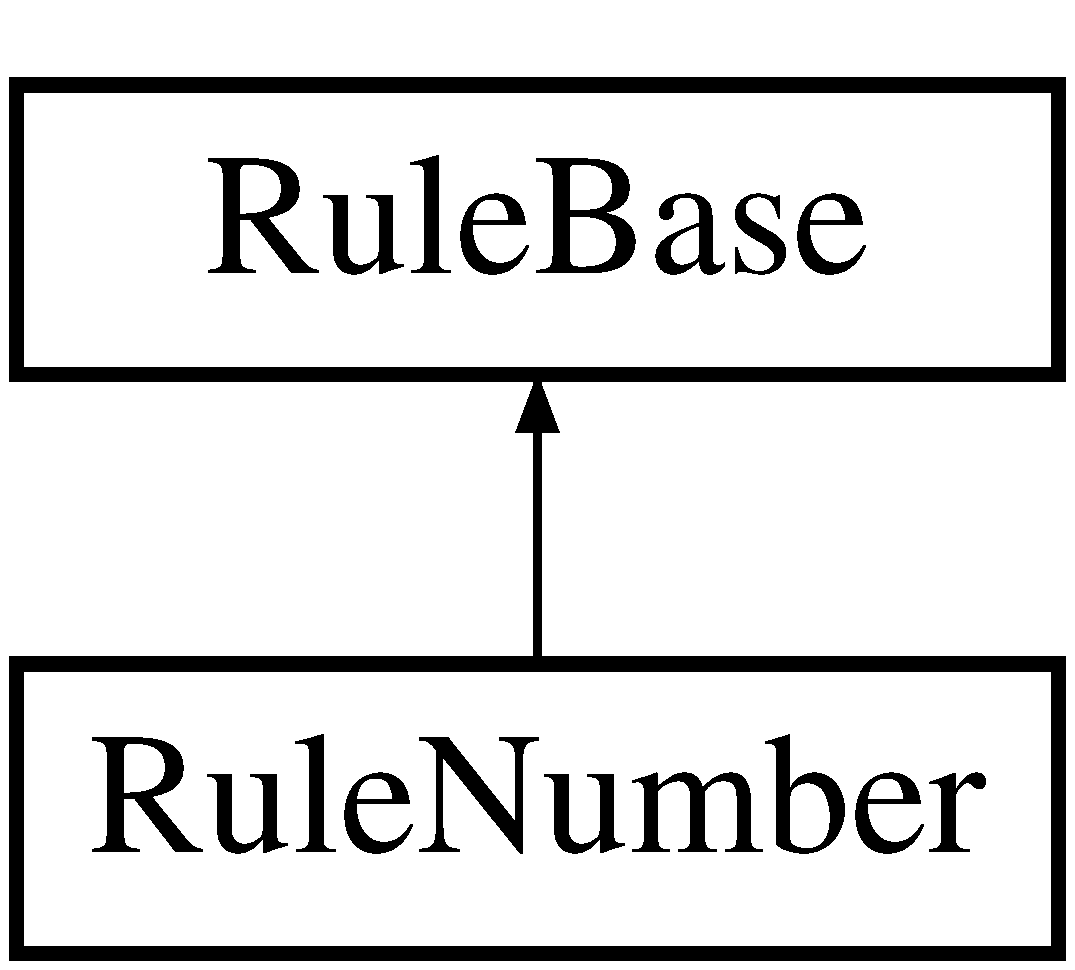
\includegraphics[height=2.000000cm]{class_rule_number}
\end{center}
\end{figure}
\subsection*{公開メンバ関数}
\begin{DoxyCompactItemize}
\item 
\hyperlink{class_rule_number_a095c5d389db211932136b53f25f39685}{\+\_\+\+\_\+construct} ()
\item 
\hyperlink{class_rule_number_afb0fafe7e02a3ae1993c01c19fad2bae}{run} ()
\end{DoxyCompactItemize}
\subsection*{その他の継承メンバ}


\subsection{詳解}
ルール:数値クラス

\begin{DoxyVersion}{バージョン}
1.\+0.\+0  U\+T\+F-\/8  2011/10/06  2011/10/19 
\end{DoxyVersion}
\begin{DoxyAuthor}{著者}
mamiya\+\_\+shou 
\end{DoxyAuthor}
\begin{DoxyCopyright}{著作権所有}
mamiya\+\_\+shou  M\+I\+T License  P\+H\+P 5.\+0 以上必須 
\end{DoxyCopyright}


\subsection{構築子と解体子}
\hypertarget{class_rule_number_a095c5d389db211932136b53f25f39685}{\index{Rule\+Number@{Rule\+Number}!\+\_\+\+\_\+construct@{\+\_\+\+\_\+construct}}
\index{\+\_\+\+\_\+construct@{\+\_\+\+\_\+construct}!Rule\+Number@{Rule\+Number}}
\subsubsection[{\+\_\+\+\_\+construct}]{\setlength{\rightskip}{0pt plus 5cm}\+\_\+\+\_\+construct (
\begin{DoxyParamCaption}
{}
\end{DoxyParamCaption}
)}}\label{class_rule_number_a095c5d389db211932136b53f25f39685}
コンストラクタ

public \begin{DoxyReturn}{戻り値}
void 
\end{DoxyReturn}


\subsection{関数詳解}
\hypertarget{class_rule_number_afb0fafe7e02a3ae1993c01c19fad2bae}{\index{Rule\+Number@{Rule\+Number}!run@{run}}
\index{run@{run}!Rule\+Number@{Rule\+Number}}
\subsubsection[{run}]{\setlength{\rightskip}{0pt plus 5cm}run (
\begin{DoxyParamCaption}
{}
\end{DoxyParamCaption}
)}}\label{class_rule_number_afb0fafe7e02a3ae1993c01c19fad2bae}
バリデートする

public \begin{DoxyReturn}{戻り値}
boolean T\+R\+U\+E(\+O\+K) / string エラーメッセージ(\+N\+G)  未入力('')の場合は\+T\+R\+U\+Eを返す 
\end{DoxyReturn}


このクラス詳解は次のファイルから抽出されました\+:\begin{DoxyCompactItemize}
\item 
Validate/rules/number.\+php\end{DoxyCompactItemize}

\hypertarget{class_rule_regular_expression}{\section{Rule\+Regular\+Expression クラス}
\label{class_rule_regular_expression}\index{Rule\+Regular\+Expression@{Rule\+Regular\+Expression}}
}
Rule\+Regular\+Expression の継承関係図\begin{figure}[H]
\begin{center}
\leavevmode
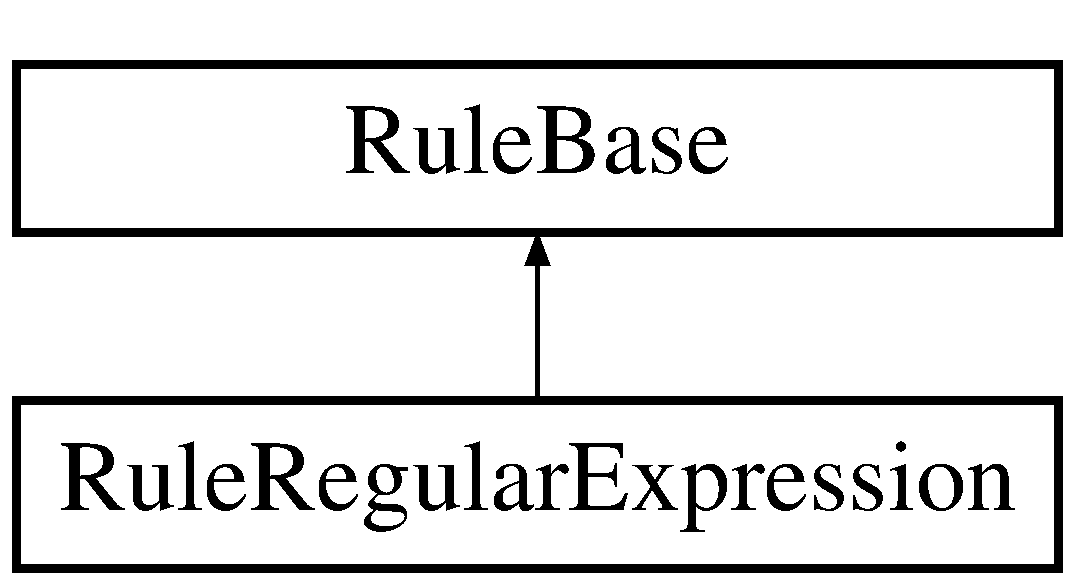
\includegraphics[height=2.000000cm]{class_rule_regular_expression}
\end{center}
\end{figure}
\subsection*{公開メンバ関数}
\begin{DoxyCompactItemize}
\item 
\hyperlink{class_rule_regular_expression_a095c5d389db211932136b53f25f39685}{\+\_\+\+\_\+construct} ()
\item 
\hyperlink{class_rule_regular_expression_afb0fafe7e02a3ae1993c01c19fad2bae}{run} ()
\end{DoxyCompactItemize}
\subsection*{その他の継承メンバ}


\subsection{詳解}
ルール:正規表現クラス

\begin{DoxyVersion}{バージョン}
1.\+0.\+0  U\+T\+F-\/8  2011/10/10  2011/10/19 
\end{DoxyVersion}
\begin{DoxyAuthor}{著者}
mamiya\+\_\+shou 
\end{DoxyAuthor}
\begin{DoxyCopyright}{著作権所有}
mamiya\+\_\+shou  M\+I\+T License  P\+H\+P 5.\+0 以上必須 
\end{DoxyCopyright}


\subsection{構築子と解体子}
\hypertarget{class_rule_regular_expression_a095c5d389db211932136b53f25f39685}{\index{Rule\+Regular\+Expression@{Rule\+Regular\+Expression}!\+\_\+\+\_\+construct@{\+\_\+\+\_\+construct}}
\index{\+\_\+\+\_\+construct@{\+\_\+\+\_\+construct}!Rule\+Regular\+Expression@{Rule\+Regular\+Expression}}
\subsubsection[{\+\_\+\+\_\+construct}]{\setlength{\rightskip}{0pt plus 5cm}\+\_\+\+\_\+construct (
\begin{DoxyParamCaption}
{}
\end{DoxyParamCaption}
)}}\label{class_rule_regular_expression_a095c5d389db211932136b53f25f39685}
コンストラクタ

public \begin{DoxyReturn}{戻り値}
void 
\end{DoxyReturn}


\subsection{関数詳解}
\hypertarget{class_rule_regular_expression_afb0fafe7e02a3ae1993c01c19fad2bae}{\index{Rule\+Regular\+Expression@{Rule\+Regular\+Expression}!run@{run}}
\index{run@{run}!Rule\+Regular\+Expression@{Rule\+Regular\+Expression}}
\subsubsection[{run}]{\setlength{\rightskip}{0pt plus 5cm}run (
\begin{DoxyParamCaption}
{}
\end{DoxyParamCaption}
)}}\label{class_rule_regular_expression_afb0fafe7e02a3ae1993c01c19fad2bae}
バリデートする

public \begin{DoxyReturn}{戻り値}
boolean T\+R\+U\+E(\+O\+K) / string エラーメッセージ(\+N\+G) 
\end{DoxyReturn}

\begin{DoxyExceptions}{例外}
{\em Exception} & validate.\+php \hyperlink{class_rule_regular_expression_afb0fafe7e02a3ae1993c01c19fad2bae}{run()}で捕捉する  未入力('')の場合は\+T\+R\+U\+Eを返す \\
\hline
\end{DoxyExceptions}


このクラス詳解は次のファイルから抽出されました\+:\begin{DoxyCompactItemize}
\item 
Validate/rules/regular\+\_\+expression.\+php\end{DoxyCompactItemize}

\hypertarget{class_rule_required}{
\section{クラス \-Rule\-Required}
\label{class_rule_required}\index{\-Rule\-Required@{\-Rule\-Required}}
}
\-Rule\-Requiredに対する継承グラフ\begin{figure}[H]
\begin{center}
\leavevmode
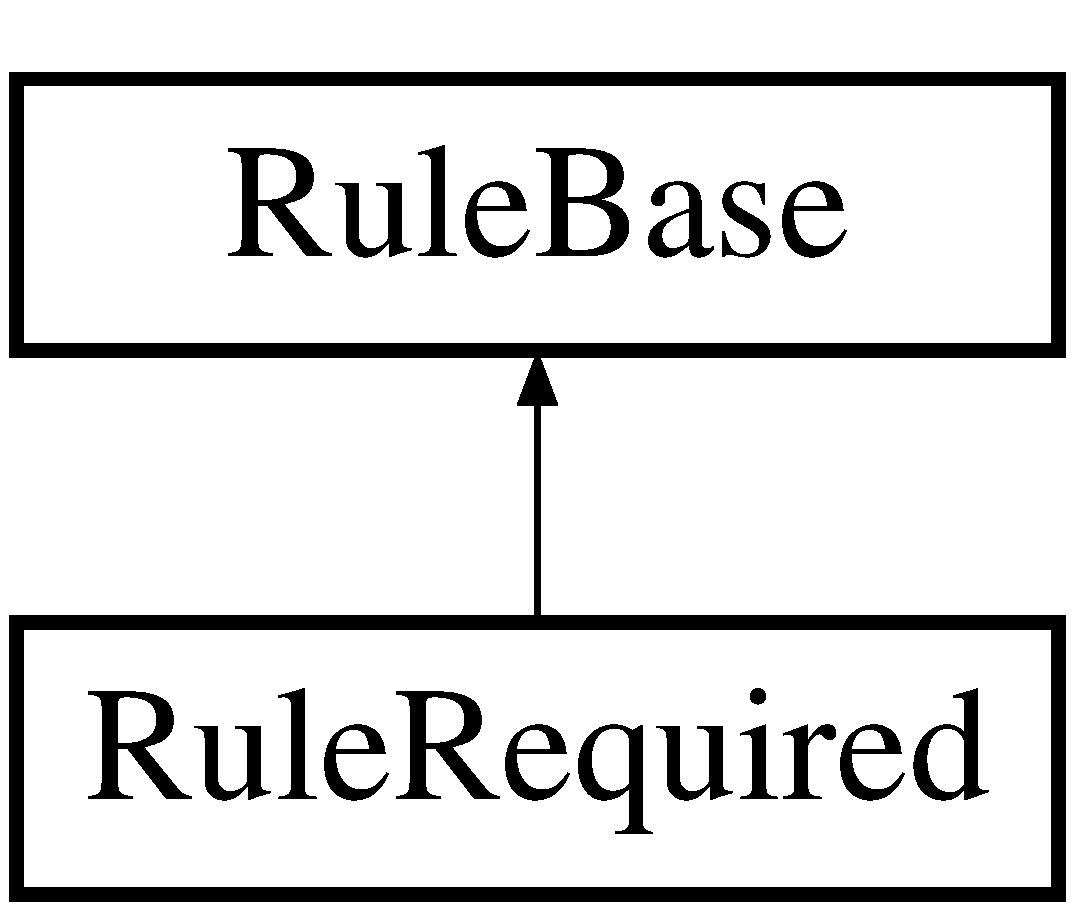
\includegraphics[height=2.000000cm]{class_rule_required}
\end{center}
\end{figure}
\subsection*{\-Public メソッド}
\begin{DoxyCompactItemize}
\item 
\hyperlink{class_rule_required_a095c5d389db211932136b53f25f39685}{\-\_\-\-\_\-construct} ()
\item 
\hyperlink{class_rule_required_afb0fafe7e02a3ae1993c01c19fad2bae}{run} ()
\end{DoxyCompactItemize}


\subsection{説明}
ルール:必須入力クラス

\begin{DoxyVersion}{バージョン}
1.\-0.\-0  \-U\-T\-F-\/8  2011/10/05  2011/10/19 
\end{DoxyVersion}
\begin{DoxyAuthor}{作者}
mamiya\-\_\-shou 
\end{DoxyAuthor}
\begin{DoxyCopyright}{\-Copyright}
mamiya\-\_\-shou  \-M\-I\-T \-License  \-P\-H\-P 5.\-0 以上必須 
\end{DoxyCopyright}


\subsection{コンストラクタとデストラクタ}
\hypertarget{class_rule_required_a095c5d389db211932136b53f25f39685}{
\index{\-Rule\-Required@{\-Rule\-Required}!\-\_\-\-\_\-construct@{\-\_\-\-\_\-construct}}
\index{\-\_\-\-\_\-construct@{\-\_\-\-\_\-construct}!RuleRequired@{\-Rule\-Required}}
\subsubsection[{\-\_\-\-\_\-construct}]{\setlength{\rightskip}{0pt plus 5cm}\-\_\-\-\_\-construct (
\begin{DoxyParamCaption}
{}
\end{DoxyParamCaption}
)}}
\label{class_rule_required_a095c5d389db211932136b53f25f39685}
コンストラクタ

public \begin{DoxyReturn}{戻り値}
void 
\end{DoxyReturn}


\subsection{関数}
\hypertarget{class_rule_required_afb0fafe7e02a3ae1993c01c19fad2bae}{
\index{\-Rule\-Required@{\-Rule\-Required}!run@{run}}
\index{run@{run}!RuleRequired@{\-Rule\-Required}}
\subsubsection[{run}]{\setlength{\rightskip}{0pt plus 5cm}run (
\begin{DoxyParamCaption}
{}
\end{DoxyParamCaption}
)}}
\label{class_rule_required_afb0fafe7e02a3ae1993c01c19fad2bae}
バリデートする

public \begin{DoxyReturn}{戻り値}
boolean \-T\-R\-U\-E(\-O\-K) / string エラーメッセージ(\-N\-G) 
\end{DoxyReturn}


\hyperlink{class_rule_base_afb0fafe7e02a3ae1993c01c19fad2bae}{\-Rule\-Base}を再定義しています。



このクラスの説明は次のファイルから生成されました\-:\begin{DoxyCompactItemize}
\item 
rules/\hyperlink{required_8php}{required.\-php}\end{DoxyCompactItemize}

\hypertarget{class_rule_select}{
\section{クラス \-Rule\-Select}
\label{class_rule_select}\index{\-Rule\-Select@{\-Rule\-Select}}
}
\-Rule\-Selectに対する継承グラフ\begin{figure}[H]
\begin{center}
\leavevmode
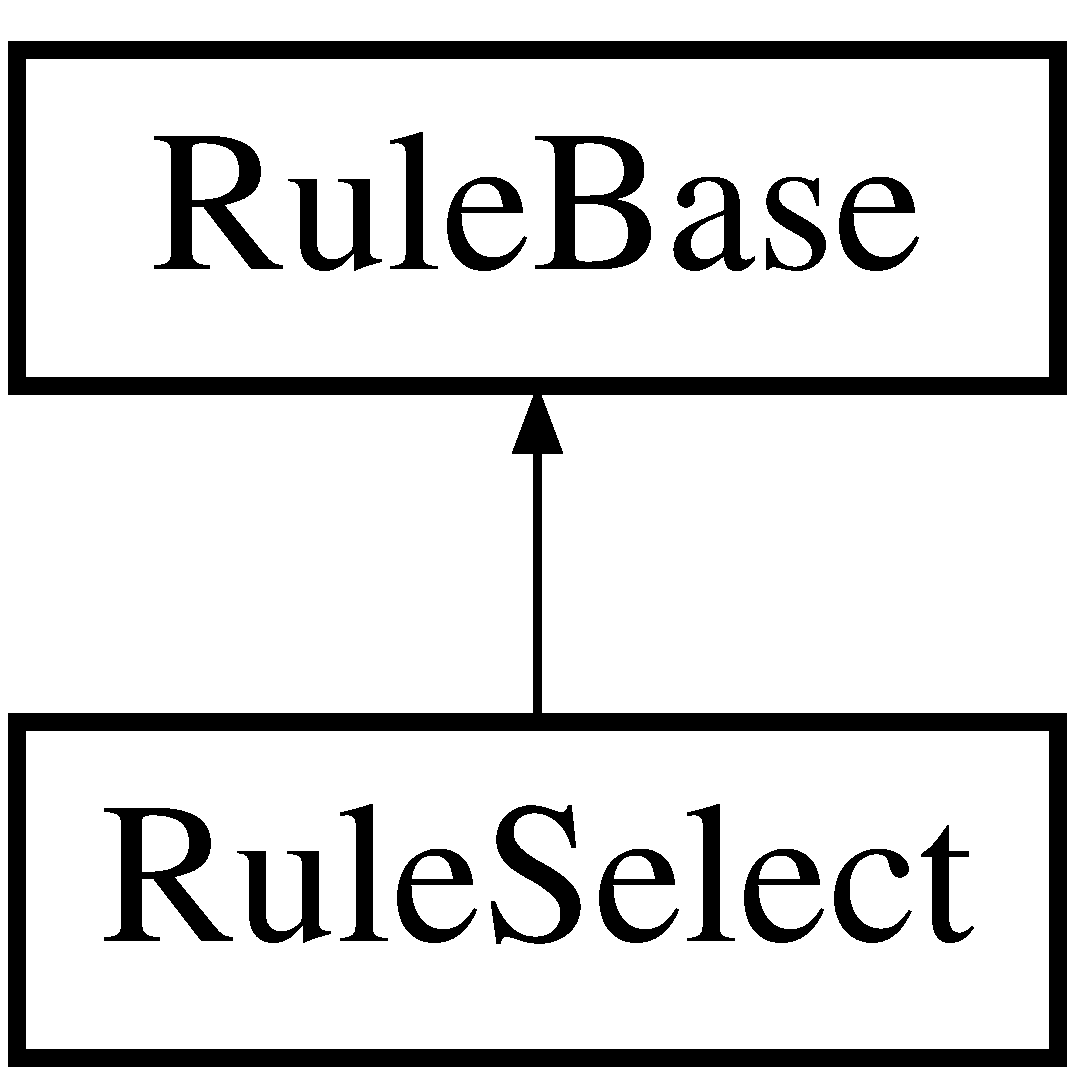
\includegraphics[height=2.000000cm]{class_rule_select}
\end{center}
\end{figure}
\subsection*{\-Public メソッド}
\begin{DoxyCompactItemize}
\item 
\hyperlink{class_rule_select_a095c5d389db211932136b53f25f39685}{\-\_\-\-\_\-construct} ()
\item 
\hyperlink{class_rule_select_afb0fafe7e02a3ae1993c01c19fad2bae}{run} ()
\end{DoxyCompactItemize}


\subsection{説明}
ルール:選択クラス

\begin{DoxyVersion}{バージョン}
1.\-0.\-0  \-U\-T\-F-\/8  2011/10/13  2011/10/19 
\end{DoxyVersion}
\begin{DoxyAuthor}{作者}
mamiya\-\_\-shou 
\end{DoxyAuthor}
\begin{DoxyCopyright}{\-Copyright}
mamiya\-\_\-shou  \-M\-I\-T \-License 
\end{DoxyCopyright}


\subsection{コンストラクタとデストラクタ}
\hypertarget{class_rule_select_a095c5d389db211932136b53f25f39685}{
\index{\-Rule\-Select@{\-Rule\-Select}!\-\_\-\-\_\-construct@{\-\_\-\-\_\-construct}}
\index{\-\_\-\-\_\-construct@{\-\_\-\-\_\-construct}!RuleSelect@{\-Rule\-Select}}
\subsubsection[{\-\_\-\-\_\-construct}]{\setlength{\rightskip}{0pt plus 5cm}\-\_\-\-\_\-construct (
\begin{DoxyParamCaption}
{}
\end{DoxyParamCaption}
)}}
\label{class_rule_select_a095c5d389db211932136b53f25f39685}
コンストラクタ

public \begin{DoxyReturn}{戻り値}
void 
\end{DoxyReturn}


\subsection{関数}
\hypertarget{class_rule_select_afb0fafe7e02a3ae1993c01c19fad2bae}{
\index{\-Rule\-Select@{\-Rule\-Select}!run@{run}}
\index{run@{run}!RuleSelect@{\-Rule\-Select}}
\subsubsection[{run}]{\setlength{\rightskip}{0pt plus 5cm}run (
\begin{DoxyParamCaption}
{}
\end{DoxyParamCaption}
)}}
\label{class_rule_select_afb0fafe7e02a3ae1993c01c19fad2bae}
バリデートする

public \begin{DoxyReturn}{戻り値}
boolean \-T\-R\-U\-E(\-O\-K) / string エラーメッセージ(\-N\-G) 
\end{DoxyReturn}

\begin{DoxyExceptions}{例外}
{\em \-Exception} & \hyperlink{validate_8php}{validate.\-php} \hyperlink{class_rule_select_afb0fafe7e02a3ae1993c01c19fad2bae}{run()}で捕捉する \\
\hline
\end{DoxyExceptions}


\hyperlink{class_rule_base_afb0fafe7e02a3ae1993c01c19fad2bae}{\-Rule\-Base}を再定義しています。



このクラスの説明は次のファイルから生成されました\-:\begin{DoxyCompactItemize}
\item 
rules/\hyperlink{select_8php}{select.\-php}\end{DoxyCompactItemize}

\hypertarget{class_rule_single}{
\section{クラス \-Rule\-Single}
\label{class_rule_single}\index{\-Rule\-Single@{\-Rule\-Single}}
}
\-Rule\-Singleに対する継承グラフ\begin{figure}[H]
\begin{center}
\leavevmode
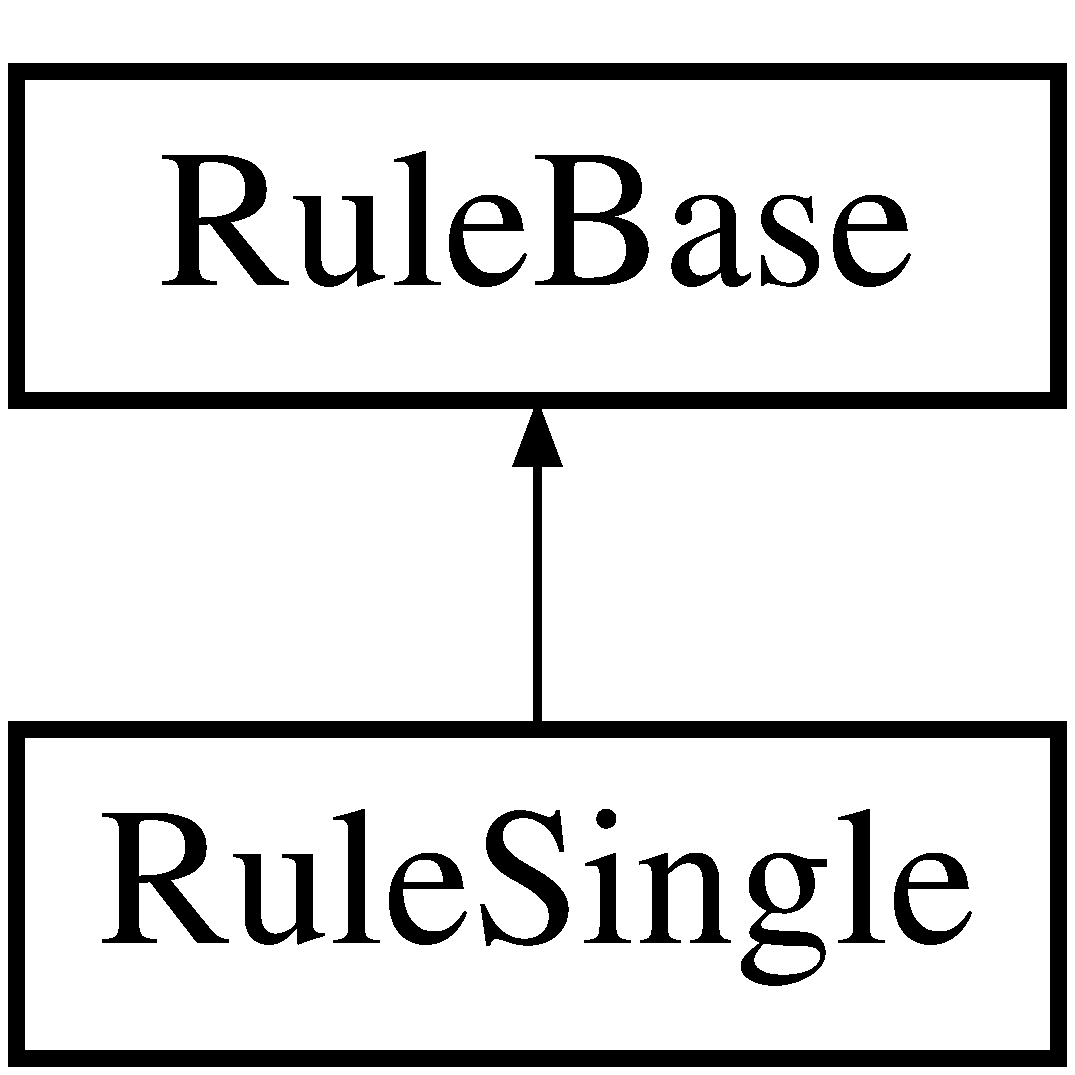
\includegraphics[height=2.000000cm]{class_rule_single}
\end{center}
\end{figure}
\subsection*{\-Public メソッド}
\begin{DoxyCompactItemize}
\item 
\hyperlink{class_rule_single_a095c5d389db211932136b53f25f39685}{\-\_\-\-\_\-construct} ()
\item 
\hyperlink{class_rule_single_afb0fafe7e02a3ae1993c01c19fad2bae}{run} ()
\end{DoxyCompactItemize}


\subsection{説明}
ルール:半角文字クラス

\begin{DoxyVersion}{バージョン}
1.\-0.\-0  \-U\-T\-F-\/8  2011/10/08  2011/10/19 
\end{DoxyVersion}
\begin{DoxyAuthor}{作者}
mamiya\-\_\-shou 
\end{DoxyAuthor}
\begin{DoxyCopyright}{\-Copyright}
mamiya\-\_\-shou  \-M\-I\-T \-License  \-P\-H\-P 5.\-0 以上必須 
\end{DoxyCopyright}


\subsection{コンストラクタとデストラクタ}
\hypertarget{class_rule_single_a095c5d389db211932136b53f25f39685}{
\index{\-Rule\-Single@{\-Rule\-Single}!\-\_\-\-\_\-construct@{\-\_\-\-\_\-construct}}
\index{\-\_\-\-\_\-construct@{\-\_\-\-\_\-construct}!RuleSingle@{\-Rule\-Single}}
\subsubsection[{\-\_\-\-\_\-construct}]{\setlength{\rightskip}{0pt plus 5cm}\-\_\-\-\_\-construct (
\begin{DoxyParamCaption}
{}
\end{DoxyParamCaption}
)}}
\label{class_rule_single_a095c5d389db211932136b53f25f39685}
コンストラクタ

public \begin{DoxyReturn}{戻り値}
void 
\end{DoxyReturn}


\subsection{関数}
\hypertarget{class_rule_single_afb0fafe7e02a3ae1993c01c19fad2bae}{
\index{\-Rule\-Single@{\-Rule\-Single}!run@{run}}
\index{run@{run}!RuleSingle@{\-Rule\-Single}}
\subsubsection[{run}]{\setlength{\rightskip}{0pt plus 5cm}run (
\begin{DoxyParamCaption}
{}
\end{DoxyParamCaption}
)}}
\label{class_rule_single_afb0fafe7e02a3ae1993c01c19fad2bae}
バリデートする

public \begin{DoxyReturn}{戻り値}
boolean \-T\-R\-U\-E(\-O\-K) / string エラーメッセージ(\-N\-G) 
\end{DoxyReturn}

\begin{DoxyExceptions}{例外}
{\em \-Exception} & \hyperlink{validate_8php}{validate.\-php} \hyperlink{class_rule_single_afb0fafe7e02a3ae1993c01c19fad2bae}{run()}で捕捉する  未入力('')の場合は\-T\-R\-U\-Eを返す \\
\hline
\end{DoxyExceptions}


\hyperlink{class_rule_base_afb0fafe7e02a3ae1993c01c19fad2bae}{\-Rule\-Base}を再定義しています。



このクラスの説明は次のファイルから生成されました\-:\begin{DoxyCompactItemize}
\item 
rules/\hyperlink{single_8php}{single.\-php}\end{DoxyCompactItemize}

\hypertarget{class_rule_tel}{\section{Rule\+Tel クラス}
\label{class_rule_tel}\index{Rule\+Tel@{Rule\+Tel}}
}
Rule\+Tel の継承関係図\begin{figure}[H]
\begin{center}
\leavevmode
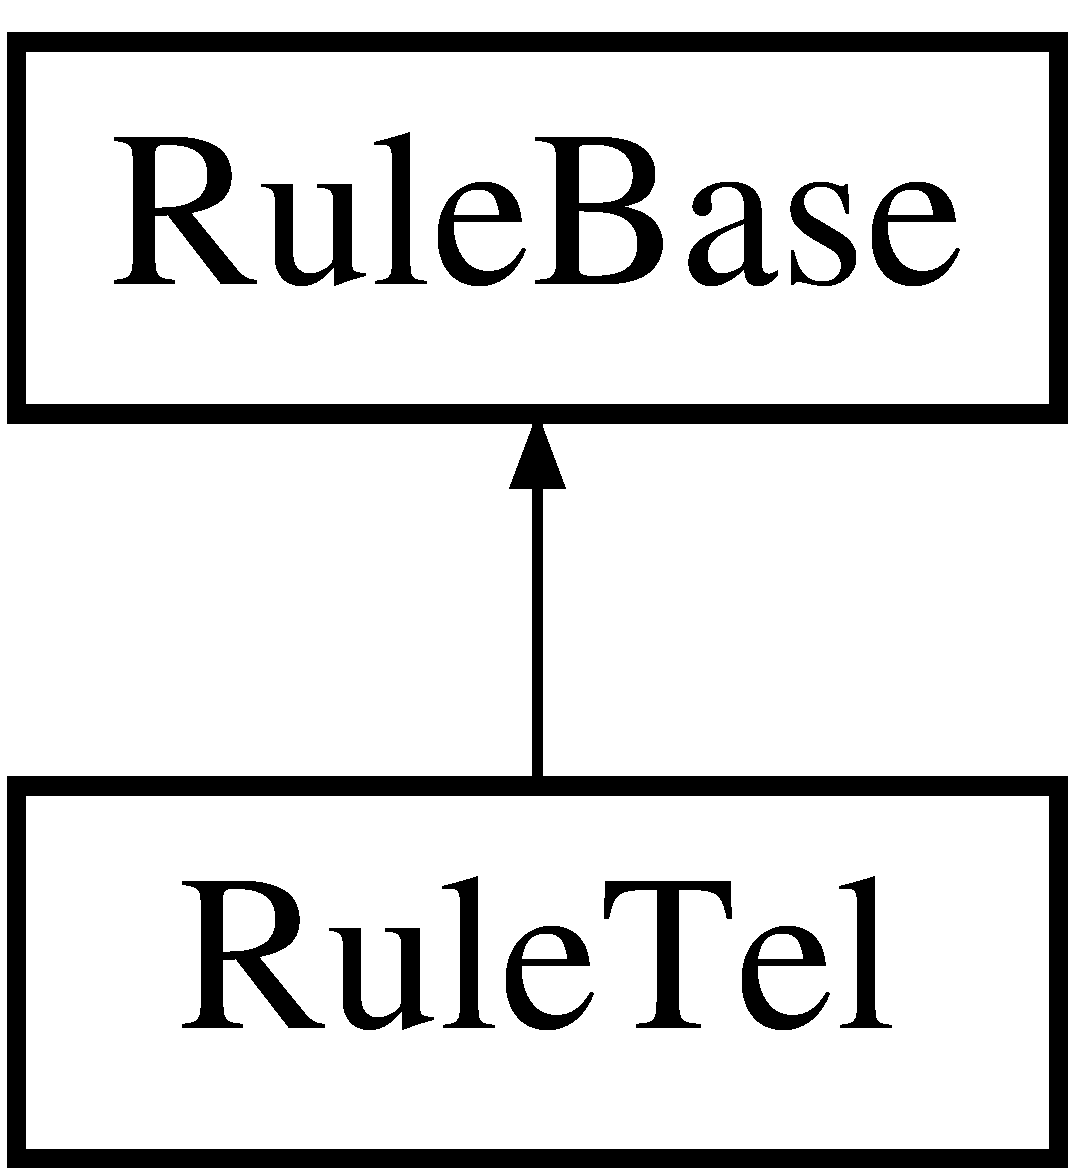
\includegraphics[height=2.000000cm]{class_rule_tel}
\end{center}
\end{figure}
\subsection*{公開メンバ関数}
\begin{DoxyCompactItemize}
\item 
\hyperlink{class_rule_tel_a095c5d389db211932136b53f25f39685}{\+\_\+\+\_\+construct} ()
\item 
\hyperlink{class_rule_tel_afb0fafe7e02a3ae1993c01c19fad2bae}{run} ()
\end{DoxyCompactItemize}
\subsection*{その他の継承メンバ}


\subsection{詳解}
ルール:電話番号クラス

\begin{DoxyVersion}{バージョン}
1.\+0.\+0  U\+T\+F-\/8  2011/10/09  2011/10/19 
\end{DoxyVersion}
\begin{DoxyAuthor}{著者}
mamiya\+\_\+shou 
\end{DoxyAuthor}
\begin{DoxyCopyright}{著作権所有}
mamiya\+\_\+shou  M\+I\+T License  P\+H\+P 5.\+0 以上必須 
\end{DoxyCopyright}


\subsection{構築子と解体子}
\hypertarget{class_rule_tel_a095c5d389db211932136b53f25f39685}{\index{Rule\+Tel@{Rule\+Tel}!\+\_\+\+\_\+construct@{\+\_\+\+\_\+construct}}
\index{\+\_\+\+\_\+construct@{\+\_\+\+\_\+construct}!Rule\+Tel@{Rule\+Tel}}
\subsubsection[{\+\_\+\+\_\+construct}]{\setlength{\rightskip}{0pt plus 5cm}\+\_\+\+\_\+construct (
\begin{DoxyParamCaption}
{}
\end{DoxyParamCaption}
)}}\label{class_rule_tel_a095c5d389db211932136b53f25f39685}
コンストラクタ

public \begin{DoxyReturn}{戻り値}
void 
\end{DoxyReturn}


\subsection{関数詳解}
\hypertarget{class_rule_tel_afb0fafe7e02a3ae1993c01c19fad2bae}{\index{Rule\+Tel@{Rule\+Tel}!run@{run}}
\index{run@{run}!Rule\+Tel@{Rule\+Tel}}
\subsubsection[{run}]{\setlength{\rightskip}{0pt plus 5cm}run (
\begin{DoxyParamCaption}
{}
\end{DoxyParamCaption}
)}}\label{class_rule_tel_afb0fafe7e02a3ae1993c01c19fad2bae}
バリデートする

public \begin{DoxyReturn}{戻り値}
boolean T\+R\+U\+E(\+O\+K) / string エラーメッセージ(\+N\+G) 
\end{DoxyReturn}

\begin{DoxyExceptions}{例外}
{\em Exception} & validate.\+php \hyperlink{class_rule_tel_afb0fafe7e02a3ae1993c01c19fad2bae}{run()}で捕捉する  未入力('')の場合は\+T\+R\+U\+Eを返す \\
\hline
\end{DoxyExceptions}


このクラス詳解は次のファイルから抽出されました\+:\begin{DoxyCompactItemize}
\item 
Validate/rules/tel.\+php\end{DoxyCompactItemize}

\hypertarget{class_rule_time}{
\section{クラス \-Rule\-Time}
\label{class_rule_time}\index{\-Rule\-Time@{\-Rule\-Time}}
}
\-Rule\-Timeに対する継承グラフ\begin{figure}[H]
\begin{center}
\leavevmode
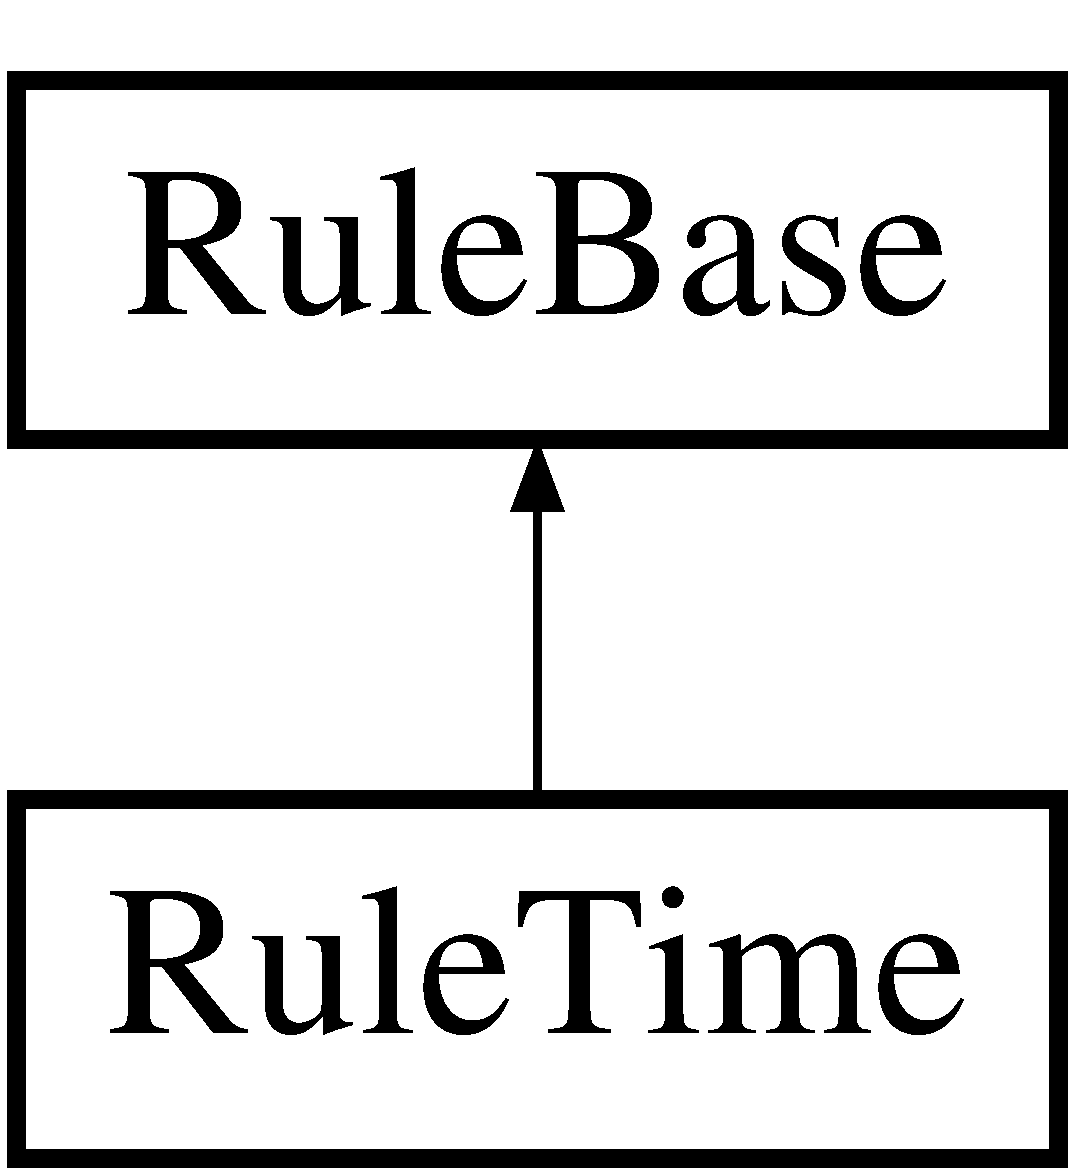
\includegraphics[height=2.000000cm]{class_rule_time}
\end{center}
\end{figure}
\subsection*{\-Public メソッド}
\begin{DoxyCompactItemize}
\item 
\hyperlink{class_rule_time_a095c5d389db211932136b53f25f39685}{\-\_\-\-\_\-construct} ()
\item 
\hyperlink{class_rule_time_afb0fafe7e02a3ae1993c01c19fad2bae}{run} ()
\end{DoxyCompactItemize}


\subsection{説明}
ルール:時刻クラス

\begin{DoxyVersion}{バージョン}
1.\-0.\-0  \-U\-T\-F-\/8  2011/10/11  2011/10/19 
\end{DoxyVersion}
\begin{DoxyAuthor}{作者}
mamiya\-\_\-shou 
\end{DoxyAuthor}
\begin{DoxyCopyright}{\-Copyright}
mamiya\-\_\-shou  \-M\-I\-T \-License  \-P\-H\-P 5.\-0 以上必須 
\end{DoxyCopyright}


\subsection{コンストラクタとデストラクタ}
\hypertarget{class_rule_time_a095c5d389db211932136b53f25f39685}{
\index{\-Rule\-Time@{\-Rule\-Time}!\-\_\-\-\_\-construct@{\-\_\-\-\_\-construct}}
\index{\-\_\-\-\_\-construct@{\-\_\-\-\_\-construct}!RuleTime@{\-Rule\-Time}}
\subsubsection[{\-\_\-\-\_\-construct}]{\setlength{\rightskip}{0pt plus 5cm}\-\_\-\-\_\-construct (
\begin{DoxyParamCaption}
{}
\end{DoxyParamCaption}
)}}
\label{class_rule_time_a095c5d389db211932136b53f25f39685}
コンストラクタ

public \begin{DoxyReturn}{戻り値}
void 
\end{DoxyReturn}


\subsection{関数}
\hypertarget{class_rule_time_afb0fafe7e02a3ae1993c01c19fad2bae}{
\index{\-Rule\-Time@{\-Rule\-Time}!run@{run}}
\index{run@{run}!RuleTime@{\-Rule\-Time}}
\subsubsection[{run}]{\setlength{\rightskip}{0pt plus 5cm}run (
\begin{DoxyParamCaption}
{}
\end{DoxyParamCaption}
)}}
\label{class_rule_time_afb0fafe7e02a3ae1993c01c19fad2bae}
バリデートする

public \begin{DoxyReturn}{戻り値}
boolean \-T\-R\-U\-E(\-O\-K) / string エラーメッセージ(\-N\-G) 
\end{DoxyReturn}

\begin{DoxyExceptions}{例外}
{\em \-Exception} & \hyperlink{validate_8php}{validate.\-php} \hyperlink{class_rule_time_afb0fafe7e02a3ae1993c01c19fad2bae}{run()}で捕捉する  未入力('')の場合は\-T\-R\-U\-Eを返す \\
\hline
\end{DoxyExceptions}


\hyperlink{class_rule_base_afb0fafe7e02a3ae1993c01c19fad2bae}{\-Rule\-Base}を再定義しています。



このクラスの説明は次のファイルから生成されました\-:\begin{DoxyCompactItemize}
\item 
rules/\hyperlink{time_8php}{time.\-php}\end{DoxyCompactItemize}

\hypertarget{class_rule_zip}{\section{Rule\+Zip クラス}
\label{class_rule_zip}\index{Rule\+Zip@{Rule\+Zip}}
}
Rule\+Zip の継承関係図\begin{figure}[H]
\begin{center}
\leavevmode
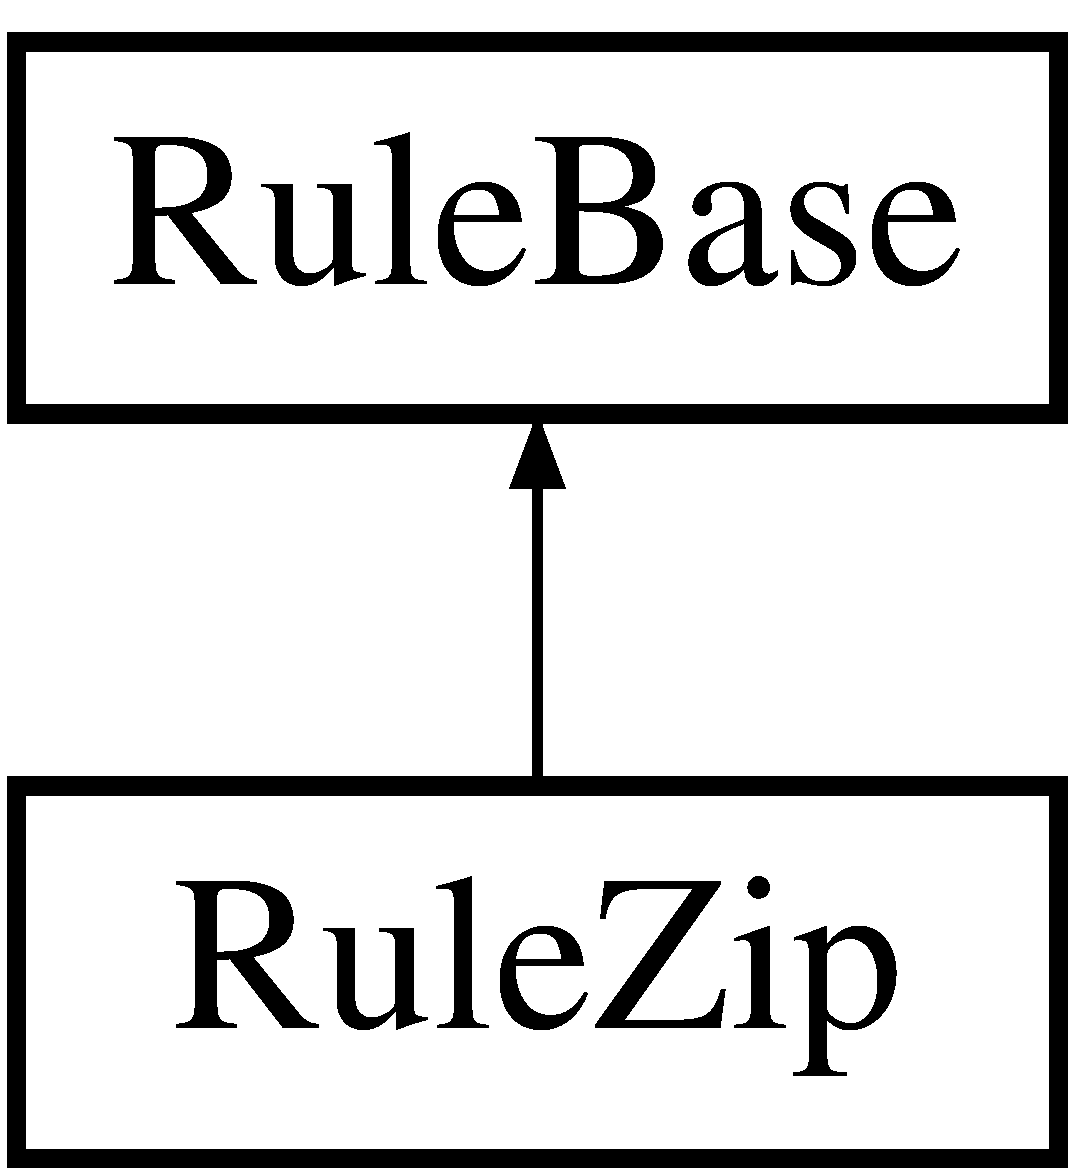
\includegraphics[height=2.000000cm]{class_rule_zip}
\end{center}
\end{figure}
\subsection*{公開メンバ関数}
\begin{DoxyCompactItemize}
\item 
\hyperlink{class_rule_zip_a095c5d389db211932136b53f25f39685}{\+\_\+\+\_\+construct} ()
\item 
\hyperlink{class_rule_zip_afb0fafe7e02a3ae1993c01c19fad2bae}{run} ()
\end{DoxyCompactItemize}
\subsection*{フィールド}
\begin{DoxyCompactItemize}
\item 
\hypertarget{class_rule_zip_ab168cbeba579bbfed03fe9f7b039d3ee}{const {\bfseries Z\+I\+P\+\_\+\+F\+I\+L\+E} = 'zip/Zip.\+php'}\label{class_rule_zip_ab168cbeba579bbfed03fe9f7b039d3ee}

\end{DoxyCompactItemize}
\subsection*{その他の継承メンバ}


\subsection{詳解}
ルール:郵便番号クラス

\begin{DoxyVersion}{バージョン}
1.\+0.\+0  U\+T\+F-\/8  2011/10/10  2011/10/19 
\end{DoxyVersion}
\begin{DoxyAuthor}{著者}
mamiya\+\_\+shou 
\end{DoxyAuthor}
\begin{DoxyCopyright}{著作権所有}
mamiya\+\_\+shou  M\+I\+T License  P\+H\+P 5.\+0 以上必須 
\end{DoxyCopyright}


\subsection{構築子と解体子}
\hypertarget{class_rule_zip_a095c5d389db211932136b53f25f39685}{\index{Rule\+Zip@{Rule\+Zip}!\+\_\+\+\_\+construct@{\+\_\+\+\_\+construct}}
\index{\+\_\+\+\_\+construct@{\+\_\+\+\_\+construct}!Rule\+Zip@{Rule\+Zip}}
\subsubsection[{\+\_\+\+\_\+construct}]{\setlength{\rightskip}{0pt plus 5cm}\+\_\+\+\_\+construct (
\begin{DoxyParamCaption}
{}
\end{DoxyParamCaption}
)}}\label{class_rule_zip_a095c5d389db211932136b53f25f39685}
コンストラクタ

public \begin{DoxyReturn}{戻り値}
void 
\end{DoxyReturn}


\subsection{関数詳解}
\hypertarget{class_rule_zip_afb0fafe7e02a3ae1993c01c19fad2bae}{\index{Rule\+Zip@{Rule\+Zip}!run@{run}}
\index{run@{run}!Rule\+Zip@{Rule\+Zip}}
\subsubsection[{run}]{\setlength{\rightskip}{0pt plus 5cm}run (
\begin{DoxyParamCaption}
{}
\end{DoxyParamCaption}
)}}\label{class_rule_zip_afb0fafe7e02a3ae1993c01c19fad2bae}
バリデートする

public \begin{DoxyReturn}{戻り値}
boolean T\+R\+U\+E(\+O\+K) / string エラーメッセージ(\+N\+G)  未入力('')の場合は\+T\+R\+U\+Eを返す 
\end{DoxyReturn}


このクラス詳解は次のファイルから抽出されました\+:\begin{DoxyCompactItemize}
\item 
Validate/rules/zip.\+php\end{DoxyCompactItemize}

\hypertarget{class_validate}{\section{Validate クラス}
\label{class_validate}\index{Validate@{Validate}}
}
\subsection*{公開メンバ関数}
\begin{DoxyCompactItemize}
\item 
\hyperlink{class_validate_affd2166b9ae24d7f6d972b6e8e27ab64}{\+\_\+\+\_\+construct} (\$requests)
\item 
\hyperlink{class_validate_a0f28658da9689c7abbfeef6620621b11}{add\+Rule} ()
\item 
\hyperlink{class_validate_a3784964295510f2bf9e3c08945073a6e}{del\+Rule} (\$name, \$type=N\+U\+L\+L)
\item 
\hyperlink{class_validate_afc81a53f0add88b49c6f84068d47987b}{copy\+Rule} (\$dest\+Name, \$src\+Name)
\item 
\hyperlink{class_validate_afb0fafe7e02a3ae1993c01c19fad2bae}{run} ()
\end{DoxyCompactItemize}
\subsection*{フィールド}
\begin{DoxyCompactItemize}
\item 
\hypertarget{class_validate_ab24faf4aa647cdcee494fc48524ad4ff}{{\bfseries \$errors}}\label{class_validate_ab24faf4aa647cdcee494fc48524ad4ff}

\item 
\hypertarget{class_validate_a233d12bd8b6d3453e9a7a3f0b8c31db2}{{\bfseries \$results}}\label{class_validate_a233d12bd8b6d3453e9a7a3f0b8c31db2}

\end{DoxyCompactItemize}


\subsection{詳解}
バリデートクラス

\begin{DoxyVersion}{バージョン}
1.\+0.\+0  U\+T\+F-\/8  2011/10/05  2011/10/19 
\end{DoxyVersion}
\begin{DoxyAuthor}{著者}
mamiya\+\_\+shou 
\end{DoxyAuthor}
\begin{DoxyCopyright}{著作権所有}
mamiya\+\_\+shou  M\+I\+T License  P\+H\+P 5.\+0 以上必須 
\end{DoxyCopyright}


\subsection{構築子と解体子}
\hypertarget{class_validate_affd2166b9ae24d7f6d972b6e8e27ab64}{\index{Validate@{Validate}!\+\_\+\+\_\+construct@{\+\_\+\+\_\+construct}}
\index{\+\_\+\+\_\+construct@{\+\_\+\+\_\+construct}!Validate@{Validate}}
\subsubsection[{\+\_\+\+\_\+construct}]{\setlength{\rightskip}{0pt plus 5cm}\+\_\+\+\_\+construct (
\begin{DoxyParamCaption}
\item[{}]{\$requests}
\end{DoxyParamCaption}
)}}\label{class_validate_affd2166b9ae24d7f6d972b6e8e27ab64}
コンストラクタ

public 
\begin{DoxyParams}[1]{引数}
array & {\em \$posts} & リクエスト配列 \\
\hline
\end{DoxyParams}
\begin{DoxyReturn}{戻り値}
void 
\end{DoxyReturn}


\subsection{関数詳解}
\hypertarget{class_validate_a0f28658da9689c7abbfeef6620621b11}{\index{Validate@{Validate}!add\+Rule@{add\+Rule}}
\index{add\+Rule@{add\+Rule}!Validate@{Validate}}
\subsubsection[{add\+Rule}]{\setlength{\rightskip}{0pt plus 5cm}add\+Rule (
\begin{DoxyParamCaption}
{}
\end{DoxyParamCaption}
)}}\label{class_validate_a0f28658da9689c7abbfeef6620621b11}
ルールを追加する

public 
\begin{DoxyParams}{引数}
{\em 可変長引数(name,type} & \mbox{[}, etc \mbox{[}, etc...\mbox{]}\mbox{]}) \\
\hline
\end{DoxyParams}
\begin{DoxyReturn}{戻り値}
boolean T\+R\+U\+E(\+O\+K) / F\+A\+L\+S\+E(\+N\+G) 
\end{DoxyReturn}
\hypertarget{class_validate_afc81a53f0add88b49c6f84068d47987b}{\index{Validate@{Validate}!copy\+Rule@{copy\+Rule}}
\index{copy\+Rule@{copy\+Rule}!Validate@{Validate}}
\subsubsection[{copy\+Rule}]{\setlength{\rightskip}{0pt plus 5cm}copy\+Rule (
\begin{DoxyParamCaption}
\item[{}]{\$dest\+Name, }
\item[{}]{\$src\+Name}
\end{DoxyParamCaption}
)}}\label{class_validate_afc81a53f0add88b49c6f84068d47987b}
ルールをコピーする

public 
\begin{DoxyParams}[1]{引数}
string & {\em \$dest\+Name} & コピー先のname値 \\
\hline
string & {\em \$src\+Name} & コピー元のname値 \\
\hline
\end{DoxyParams}
\begin{DoxyReturn}{戻り値}
boolean T\+R\+U\+E(\+O\+K) / F\+A\+L\+S\+E(\+N\+G) 
\end{DoxyReturn}
\hypertarget{class_validate_a3784964295510f2bf9e3c08945073a6e}{\index{Validate@{Validate}!del\+Rule@{del\+Rule}}
\index{del\+Rule@{del\+Rule}!Validate@{Validate}}
\subsubsection[{del\+Rule}]{\setlength{\rightskip}{0pt plus 5cm}del\+Rule (
\begin{DoxyParamCaption}
\item[{}]{\$name, }
\item[{}]{\$type = {\ttfamily NULL}}
\end{DoxyParamCaption}
)}}\label{class_validate_a3784964295510f2bf9e3c08945073a6e}
ルールを削除する

public 
\begin{DoxyParams}[1]{引数}
string & {\em \$name} & name値 \\
\hline
string & {\em \$type} & ルール名 \\
\hline
\end{DoxyParams}
\begin{DoxyReturn}{戻り値}
boolean T\+R\+U\+E(\+O\+K) / F\+A\+L\+S\+E(\+N\+G) 
\end{DoxyReturn}
\hypertarget{class_validate_afb0fafe7e02a3ae1993c01c19fad2bae}{\index{Validate@{Validate}!run@{run}}
\index{run@{run}!Validate@{Validate}}
\subsubsection[{run}]{\setlength{\rightskip}{0pt plus 5cm}run (
\begin{DoxyParamCaption}
{}
\end{DoxyParamCaption}
)}}\label{class_validate_afb0fafe7e02a3ae1993c01c19fad2bae}
バリデーションを実行する

public \begin{DoxyReturn}{戻り値}
boolean T\+R\+U\+E(エラー無し) / F\+A\+L\+S\+E(エラー有り) 
\end{DoxyReturn}


このクラス詳解は次のファイルから抽出されました\+:\begin{DoxyCompactItemize}
\item 
Validate/Validate.\+php\end{DoxyCompactItemize}

\hypertarget{class_zip}{
\section{クラス \-Zip}
\label{class_zip}\index{\-Zip@{\-Zip}}
}
\subsection*{\-Public メソッド}
\begin{DoxyCompactItemize}
\item 
\hyperlink{class_zip_a095c5d389db211932136b53f25f39685}{\-\_\-\-\_\-construct} ()
\item 
\hyperlink{class_zip_a1b4e2431640c8db17a2891014cca7860}{search} (\$zip, \$is\-New=true)
\end{DoxyCompactItemize}
\subsection*{\-Private メソッド}
\begin{DoxyCompactItemize}
\item 
\hyperlink{class_zip_ac5d3ce0d7d41fdbdabcdd5e9bde7a521}{\-\_\-check\-Format\-New} (\&\$zip)
\item 
\hyperlink{class_zip_aa55051f7b8c754f92b414a6e1be66c09}{\-\_\-check\-Format\-Old} (\&\$zip)
\item 
\hyperlink{class_zip_ab38ef87cc1c3acd5d4c8ad5632691fc9}{\-\_\-get\-Csv\-All} (\$csv\-Path, \$to\-Enc=\hyperlink{zip_2_zip_8php_a04041db498ce35468b792db6570fe163}{\-D\-E\-S\-C\-\_\-\-C\-H\-A\-R\-S\-E\-T}, \$from\-Enc=\hyperlink{zip_2_zip_8php_a6917e80f882a8e319e4d9760052bc8c4}{\-S\-R\-C\-\_\-\-C\-H\-A\-R\-S\-E\-T})
\end{DoxyCompactItemize}


\subsection{コンストラクタとデストラクタ}
\hypertarget{class_zip_a095c5d389db211932136b53f25f39685}{
\index{\-Zip@{\-Zip}!\-\_\-\-\_\-construct@{\-\_\-\-\_\-construct}}
\index{\-\_\-\-\_\-construct@{\-\_\-\-\_\-construct}!Zip@{\-Zip}}
\subsubsection[{\-\_\-\-\_\-construct}]{\setlength{\rightskip}{0pt plus 5cm}\-\_\-\-\_\-construct (
\begin{DoxyParamCaption}
{}
\end{DoxyParamCaption}
)}}
\label{class_zip_a095c5d389db211932136b53f25f39685}
コンストラクタ 

\subsection{関数}
\hypertarget{class_zip_ac5d3ce0d7d41fdbdabcdd5e9bde7a521}{
\index{\-Zip@{\-Zip}!\-\_\-check\-Format\-New@{\-\_\-check\-Format\-New}}
\index{\-\_\-check\-Format\-New@{\-\_\-check\-Format\-New}!Zip@{\-Zip}}
\subsubsection[{\-\_\-check\-Format\-New}]{\setlength{\rightskip}{0pt plus 5cm}\-\_\-check\-Format\-New (
\begin{DoxyParamCaption}
\item[{\&\$}]{zip}
\end{DoxyParamCaption}
)\hspace{0.3cm}{\ttfamily  \mbox{[}private\mbox{]}}}}
\label{class_zip_ac5d3ce0d7d41fdbdabcdd5e9bde7a521}
郵便番号(現行)の形式をチェックする


\begin{DoxyParams}[1]{引数}
string & {\em \&\$zip} & 郵便番号 \\
\hline
\end{DoxyParams}
\begin{DoxyReturn}{戻り値}
boolean true(\-O\-K) / false(\-N\-G)  郵便番号の形式は「半角数字7桁、または4文字目が区切り文字の8桁」 
\end{DoxyReturn}
\hypertarget{class_zip_aa55051f7b8c754f92b414a6e1be66c09}{
\index{\-Zip@{\-Zip}!\-\_\-check\-Format\-Old@{\-\_\-check\-Format\-Old}}
\index{\-\_\-check\-Format\-Old@{\-\_\-check\-Format\-Old}!Zip@{\-Zip}}
\subsubsection[{\-\_\-check\-Format\-Old}]{\setlength{\rightskip}{0pt plus 5cm}\-\_\-check\-Format\-Old (
\begin{DoxyParamCaption}
\item[{\&\$}]{zip}
\end{DoxyParamCaption}
)\hspace{0.3cm}{\ttfamily  \mbox{[}private\mbox{]}}}}
\label{class_zip_aa55051f7b8c754f92b414a6e1be66c09}
郵便番号(旧式)の形式をチェックする


\begin{DoxyParams}[1]{引数}
string & {\em \&\$zip} & 郵便番号 \\
\hline
\end{DoxyParams}
\begin{DoxyReturn}{戻り値}
boolean true(\-O\-K) / false(\-N\-G)  郵便番号の形式は「半角数字3桁、または5桁」 
\end{DoxyReturn}
\hypertarget{class_zip_ab38ef87cc1c3acd5d4c8ad5632691fc9}{
\index{\-Zip@{\-Zip}!\-\_\-get\-Csv\-All@{\-\_\-get\-Csv\-All}}
\index{\-\_\-get\-Csv\-All@{\-\_\-get\-Csv\-All}!Zip@{\-Zip}}
\subsubsection[{\-\_\-get\-Csv\-All}]{\setlength{\rightskip}{0pt plus 5cm}\-\_\-get\-Csv\-All (
\begin{DoxyParamCaption}
\item[{\$}]{csv\-Path, }
\item[{\$}]{to\-Enc = {\ttfamily {\bf \-D\-E\-S\-C\-\_\-\-C\-H\-A\-R\-S\-E\-T}}, }
\item[{\$}]{from\-Enc = {\ttfamily {\bf \-S\-R\-C\-\_\-\-C\-H\-A\-R\-S\-E\-T}}}
\end{DoxyParamCaption}
)\hspace{0.3cm}{\ttfamily  \mbox{[}private\mbox{]}}}}
\label{class_zip_ab38ef87cc1c3acd5d4c8ad5632691fc9}
\-C\-S\-Vファイルから全情報を読み取る


\begin{DoxyParams}[1]{引数}
string & {\em \$csv\-Path} & \-C\-S\-Vファイルパス \\
\hline
string & {\em \$to\-Enc} & 変換先の文字コード \\
\hline
string & {\em \$from\-Enc} & 変換元の文字コード \\
\hline
\end{DoxyParams}
\begin{DoxyReturn}{戻り値}
array object 結果オブジェクト配列(\-O\-K) / \-F\-A\-L\-S\-E(\-N\-G)
\end{DoxyReturn}
\mbox{[}検索結果情報\mbox{]}
\begin{DoxyItemize}
\item 成功時 \mbox{[}name\mbox{]}=$>$ アプリケーション名称 \mbox{[}version\mbox{]}=$>$ アプリケーションのバージョン \mbox{[}request\-\_\-url\mbox{]}=$>$ リクエスト\-U\-R\-L \mbox{[}request\-\_\-zip\-\_\-num\mbox{]}=$>$ リクエストされた郵便番号 \mbox{[}request\-\_\-zip\-\_\-version\mbox{]}=$>$リクエストされた郵便番号形式(0 = 7桁, 1 = 3 or 5桁, なし = none) \mbox{[}result\-\_\-code\mbox{]}=$>$ 結果コード(正常時 = 1, エラー時 = 0) \mbox{[}result\-\_\-zip\-\_\-num\mbox{]}=$>$ 検索した郵便番号 \mbox{[}result\-\_\-zip\-\_\-version\mbox{]}=$>$ 検索した郵便番号形式(0 = 7桁, 1 = 3 or 5桁) \mbox{[}result\-\_\-values\-\_\-count\mbox{]}=$>$該当した住所情報の数。 (追加情報) \mbox{[}try\-Cnt\mbox{]}=$>$ 試行回数 \mbox{[}load\-Time\mbox{]}=$>$ 読み込み時間(マイクロ秒)
\end{DoxyItemize}


\begin{DoxyItemize}
\item 失敗時(count\-:8) \mbox{[}name\mbox{]}=$>$ アプリケーション名称 \mbox{[}version\mbox{]}=$>$ アプリケーションのバージョン \mbox{[}request\-\_\-url\mbox{]}=$>$ リクエスト\-U\-R\-L \mbox{[}request\-\_\-zip\-\_\-num\mbox{]}=$>$ リクエストされた郵便番号 \mbox{[}request\-\_\-zip\-\_\-version\mbox{]}=$>$リクエストされた郵便番号形式(0 = 7桁, 1 = 3 or 5桁, なし = none) \mbox{[}result\-\_\-code\mbox{]}=$>$ 結果コード(正常時 = 1, エラー時 = 0) \mbox{[}error\-\_\-code\mbox{]}=$>$ エラーコード \mbox{[}error\-\_\-note\mbox{]}=$>$ エラー内容
\end{DoxyItemize}

\mbox{[}住所情報\mbox{]}:ヒットした場合 \mbox{[}state\-\_\-kana\mbox{]}=$>$ 都道府県カナ \mbox{[}city\-\_\-kana\mbox{]}=$>$ 市区町村カナ \mbox{[}address\-\_\-kana\mbox{]}=$>$ 住所カナ \mbox{[}company\-\_\-kana\mbox{]}=$>$ 事業所カナ \mbox{[}state\mbox{]}=$>$ \char`\"{}熊本県\char`\"{} 都道府県 \mbox{[}city\mbox{]}=$>$ \char`\"{}八代市\char`\"{} 市区町村 \mbox{[}address\mbox{]}=$>$ 住所 \mbox{[}company\mbox{]}=$>$ 事業所 (※該当情報が存在しない場合、「none」がセットされます。) \hypertarget{class_zip_a1b4e2431640c8db17a2891014cca7860}{
\index{\-Zip@{\-Zip}!search@{search}}
\index{search@{search}!Zip@{\-Zip}}
\subsubsection[{search}]{\setlength{\rightskip}{0pt plus 5cm}search (
\begin{DoxyParamCaption}
\item[{\$}]{zip, }
\item[{\$}]{is\-New = {\ttfamily true}}
\end{DoxyParamCaption}
)}}
\label{class_zip_a1b4e2431640c8db17a2891014cca7860}
郵便番号検索を行う


\begin{DoxyParams}[1]{引数}
string & {\em \$zip} & 郵便番号 \\
\hline
boolean & {\em \$is\-New} & true \-:現行郵便番号(7桁) false \-:旧式郵便番号(3桁 or 5桁) \\
\hline
\end{DoxyParams}
\begin{DoxyReturn}{戻り値}
boolean 結果オブジェクト配列(\-O\-K) / \-F\-A\-L\-S\-E(\-N\-G) 
\end{DoxyReturn}


このクラスの説明は次のファイルから生成されました\-:\begin{DoxyCompactItemize}
\item 
rules/zip/\hyperlink{zip_2_zip_8php}{\-Zip.\-php}\end{DoxyCompactItemize}

%--- End generated contents ---

% Index
\newpage
\phantomsection
\addcontentsline{toc}{chapter}{索引}
\printindex

\end{document}
